\documentclass[10pt]{beamer}
\usepackage[utf8]{inputenc}
\usepackage[french]{babel}
\usepackage[T1]{fontenc}
\usepackage{beamerthemesplit}
\usepackage{graphics,epsfig, subfigure}
\usepackage{url}
\usepackage{siunitx}
\usepackage{fourier}
\usepackage{tikz}
\usepackage{numprint}

\DeclareSIUnit\year{yr}

\definecolor{jd_blue0}{rgb}{0.51,0.34,1.00}
\definecolor{jdbishop}{rgb}{0.27,0.14,0.29}
\definecolor{jddarkbl}{rgb}{0.18,0.14,0.29}
\definecolor{jd_brown}{rgb}{0.29,0.14,0.14}
\definecolor{jd_green}{HTML}{096F35}
\definecolor{jdorange}{rgb}{1.00,0.55,0.00}
\definecolor{jdredred}{rgb}{0.50,0.00,0.00}
\definecolor{SchoolColor}{rgb}{0.145,0.666,1}
\definecolor{pheniics}{HTML}{1a899c}
\definecolor{pheniics_purple}{HTML}{64003d}
\definecolor{chaptercolor}{gray}{0.8}
\mode<presentation>
{  \usetheme{PaloAlto}

  \setbeamercolor{palette primary}{bg=pheniics,fg=white}
  \setbeamercolor{palette secondary}{bg=pheniics_purple,fg=white}
  \setbeamercolor{palette tertiary}{bg=pheniics_purple,fg=white}
  \setbeamercolor{palette quaternary}{bg=pheniics_purple,fg=white}
  \setbeamercolor{palette sidebar primary}{fg=white}
  \setbeamercolor{palette sidebar secondary}{fg=white}
  \setbeamercolor{palette sidebar tertiary}{fg=pheniics_purple}
  \setbeamercolor{palette sidebar quaternary}{fg=pheniics_purple}
  \setbeamercolor{structure}{fg=pheniics} % itemize, enumerate, etc
  \setbeamercolor{section in toc}{fg=black}

  \useinnertheme{circles}
  \usefonttheme[onlymath]{serif}
  \setbeamercovered{transparent}
  \setbeamertemplate{blocks}[rounded][shadow=true]
  \setbeamertemplate{navigation symbols}{}
  \addtobeamertemplate{footline}{
    \usebeamercolor[fg]{author in sidebar}
    \vskip-1cm\hskip15pt
    \insertframenumber\,/\,\inserttotalframenumber\kern1em\vskip2pt%
  }
}
\setbeamercovered{invisible}
%\setbeamertemplate{background}{\includegraphics[width=1\textwidth]{natfak_baggrund.pdf}}

\graphicspath{{../Chapitre_1/pictures/}{../Chapitre_2/pictures/}{../Chapitre_3/pictures/}{../Chapitre_4/pictures/}{../Chapitre_5/pictures/}{../Front-back_covers/images/}{pictures/}}
 
\logo{
\includegraphics[width=1.5cm]{logo_CEA.png}}
\title[Le projet WA105]{Le projet WA105 : un prototype de Chambre à Projection Temporelle à Argon Liquide Diphasique utilisant des détecteurs LEMs}
\author{Présenté par \\ \textbf{Philippe Cotte} \\ \vspace{0.3cm} Sous la direction de \\ \textbf{E. Mazzucato}\vspace{-0.2cm}}
\institute{CEA Paris-Saclay \\ Université Paris-Saclay\vspace{-0.2cm}}
\date{\vspace{-0.2cm}17 Septembre 2019}

\def\TOO{\SI{4}{\tonne}}
\def\SSS{\SI{300}{\tonne}}
\def\threeL{\SI{3}{\liter}}
\def\dune{DU$\nu$E}
\def\checkmark{\tikz\fill[scale=0.4](0,.35) -- (.25,0) -- (1,.7) -- (.25,.15) -- cycle;}

\newenvironment{specialframe}
{
    \begingroup
    \advance\textwidth2cm % see beamerthemeGoettingen.sty for the number
    \hsize\textwidth
    \columnwidth\textwidth
    \begin{frame}[plain]
}
{
    \end{frame}
    \endgroup
}


\begin{document}

    {
        \usebackgroundtemplate{
\includegraphics[width=\paperwidth]{./pictures/1.pdf}}
        \begin{specialframe}
            \vspace{2cm}\hspace*{-1.8cm}\parbox[t]{\textwidth}{\titlepage}
        \end{specialframe}
    }
    \begin{specialframe}{Table des matières}
        \tableofcontents[hideallsubsections]
    \end{specialframe}

  \setcounter{framenumber}{0}
    {
    	\usebackgroundtemplate{
\includegraphics[width=\paperwidth]{./pictures/1.pdf}}
        \begin{specialframe}
            \vspace{2cm}\hspace*{-1.8cm}\parbox[t]{\textwidth}{
                \begin{center}
                    \begin{Huge}
                            \textcolor{pheniics_purple}{\textbf{Contexte}}
                    \end{Huge}
                \end{center}
            }
        \end{specialframe}
    }

  \section{Contexte}
    
    \begin{frame}{La plateforme neutrino du CERN}{ProtoDU$\nu$-SP et WA105/ProtoDU$\nu$-DP}
        \begin{columns}
            \begin{column}{0.5\textwidth}
                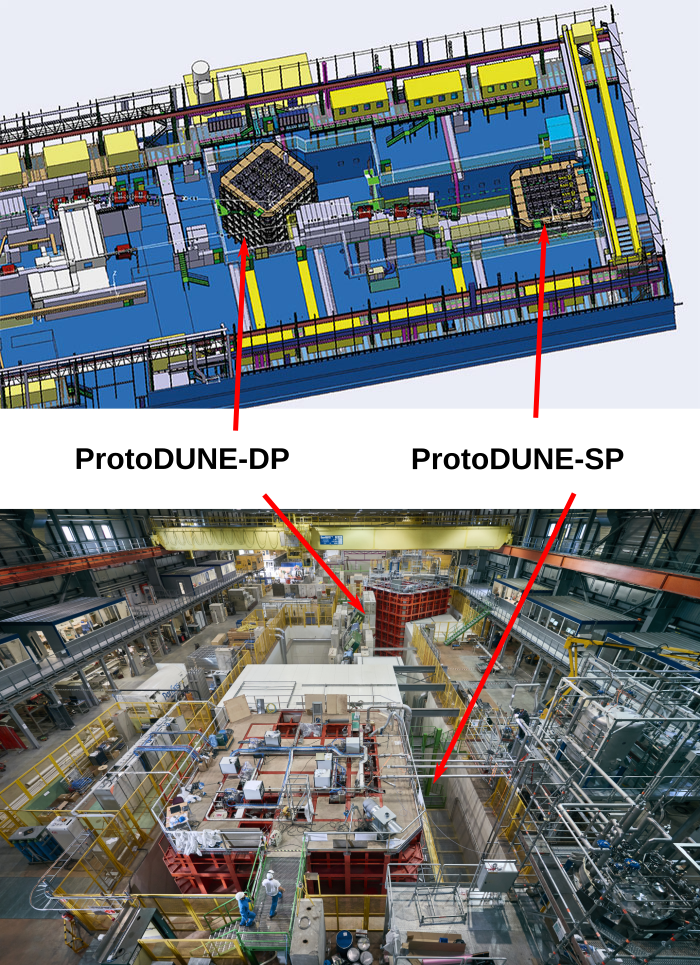
\includegraphics[height=0.9\textheight]{./pictures/neutrino_platform.png}
            \end{column}
            \begin{column}{0.5\textwidth}
                \begin{scriptsize}
                    Stratégie Européenne de physique des particules de 2013 : implication du CERN dans la recherche mondiale en physique des neutrinos : \\ $\Rightarrow$ Extension du hall de test en faisceau du site de Prévessin.\vspace{0.4cm}
                    \begin{itemize}
                        \item Prototypage de \textbf{Chambres à Projection Temporelle à Argon Liquide} : ProtoDU$\nu$-SP et \textcolor{red}{WA105/ProtoDU$\nu$-DP}
                        \item Technologie choisie pour la future expérience d'oscillation des neutrinos DU$\nu$E
                        \item Tests en faisceaux et/ou en cosmiques
                    \end{itemize}
                \end{scriptsize}
            \end{column}
        \end{columns}
    \end{frame}
        
    \subsection{DU$\nu$E}
        
    \begin{frame}{Oscillations des neutrinos : les grandes inconnues}
        \begin{columns}
            \begin{column}{0.5\textwidth}
                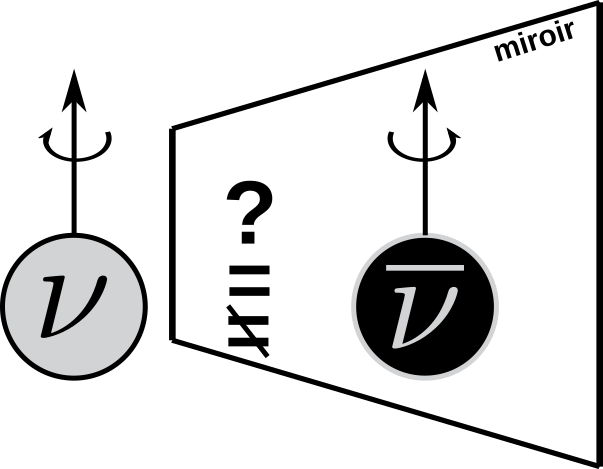
\includegraphics[width=0.8\textwidth]{./pictures/CP_schema.png}\\
                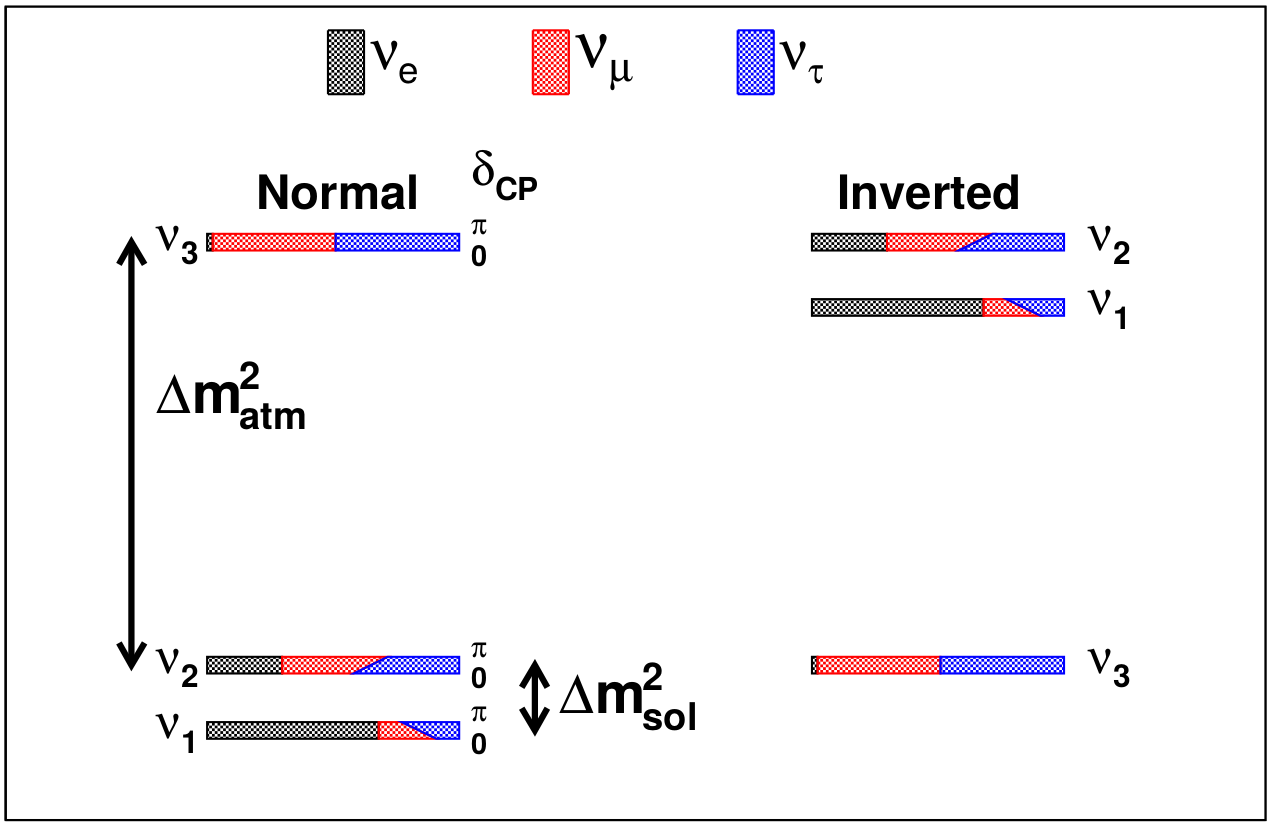
\includegraphics[width=\textwidth]{mass_hierarchy.png}
            \end{column}
            \begin{column}{0.5\textwidth}
                \begin{scriptsize}
                    \begin{itemize}
                        \item La symétrie CP est-elle violée dans le secteur leptonique?  \\ $\Rightarrow$ Pourrait expliquer l'asymétrie matière-antimatière de l'univers
                        \item Quel est l'ordre des masses des neutrinos?  \\ $\Rightarrow$ Contrainte sur certaines théories au delà du modèle standard 
                    \end{itemize}
                    \vspace{0.4cm}
                    \textbf{Connaissances actuelles :}
                \end{scriptsize}
                \begin{itemize}
                    \item \begin{scriptsize}$\delta_{CP} \ne 0$ ou $\pi$ à $2\sigma$ (i.e CP semble violée)\end{scriptsize} \\  \tiny{T2K, Physical Review Letters 121.17 (oct. 2018)}
                    \item \begin{scriptsize}3$\sigma$ en faveur de l'ordre des masses normal\end{scriptsize} \\ \tiny{NO$\nu$A, Physics Letters B 782 (juil. 2018), p. 633–640}
                \end{itemize}
            \end{column}
        \end{columns}
    \end{frame}

    \begin{frame}{DU$\nu$E : Deep Underground Neutrino Experiment}{Une expérience d'oscillation de neutrinos d'accélérateur à longue ligne de base}
        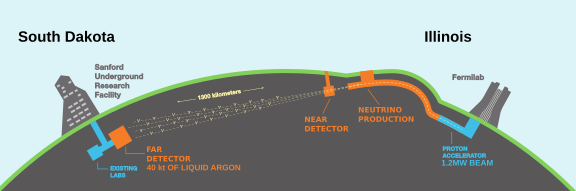
\includegraphics[width=\textwidth]{./pictures/dune.png}\\
        \begin{scriptsize}
        \vspace{0.4cm}
        \begin{columns}
            \begin{column}{0.75\textwidth}
                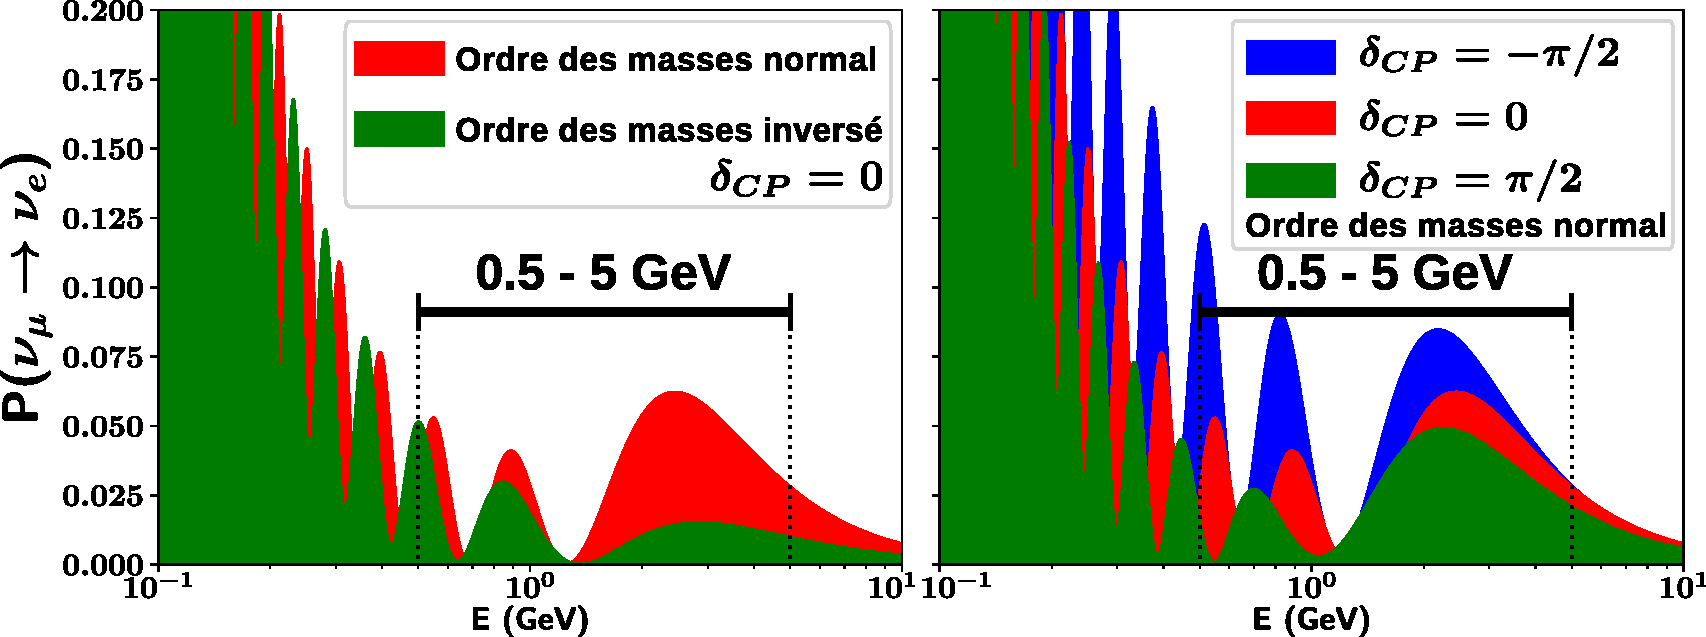
\includegraphics[width=\textwidth]{numu-nue-vs-E-MH-CP.pdf}
            \end{column}
            \hspace{-0.5cm}
            \begin{column}{0.35\textwidth}
                 \begin{itemize}
                     \item Les $\nu_{\mu}$ initiaux ont une probabilité $P(\nu_{\mu}\to\nu_e)$ d'être des $\nu_e$ à l'arrivée
                     \item \textcolor{red}{$P(\nu_{\mu}\to\nu_e)$} vs $E$ dépend de \textcolor{red}{$\delta_{CP}$} et de l'\textcolor{red}{ordre des masses}.
                     \item Fin 2026 : 7 ans de faisceau de $\nu_{\mu}$ puis 7 ans de faisceau $\overline{\nu}_{\mu}$.
                 \end{itemize}
            \end{column}
        \end{columns}
%            \centering
%            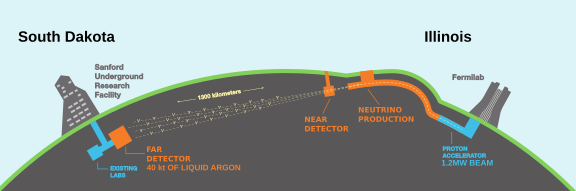
\includegraphics[width=\textwidth]{./pictures/dune.png}\\
%            \vspace{0.4cm}
%            \begin{figure}[htpb]
%              \begin{subfigure}[t]{0.49\textwidth}
%                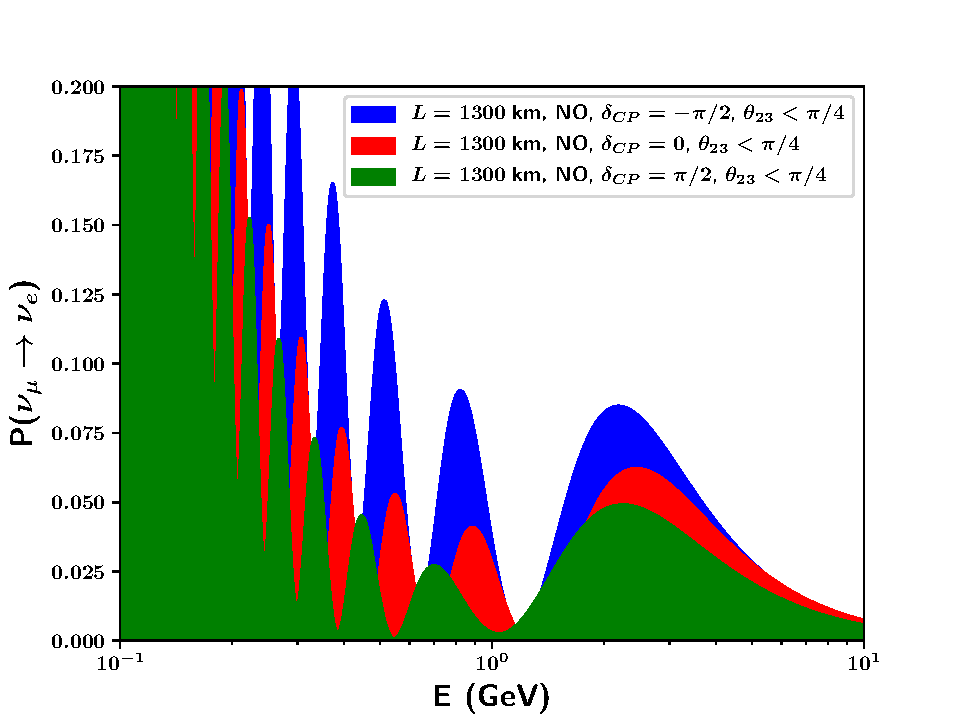
\includegraphics[width=\textwidth,keepaspectratio]{numu-nue-vs-E-cp.pdf}
%              \end{subfigure}\hfill
%              \begin{subfigure}[t]{0.49\textwidth}
%                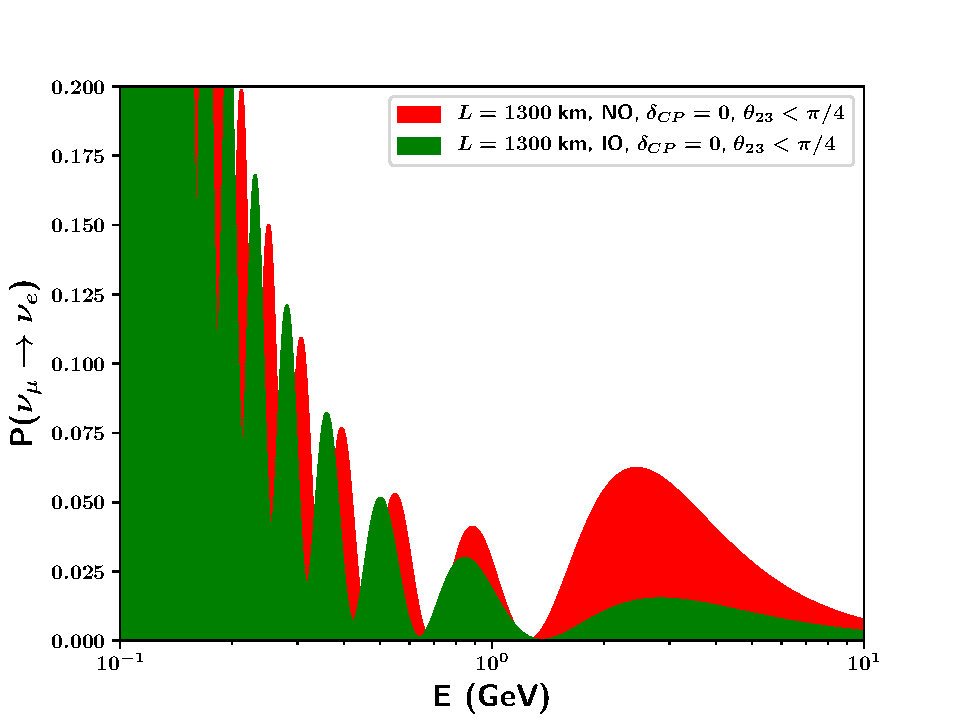
\includegraphics[width=\textwidth,keepaspectratio]{numu-nue-vs-E-MH.pdf}
%              \end{subfigure}
%%                \caption[Probabilité de changement de saveur en fonction de $E$ à \SI{1300}{\kilo\meter}]{\label{fig::two_unknown_effects}Probabilité de changement de saveur en fonction de $E$ à \SI{1300}{\kilo\meter}. Le graphe de gauche montre l'impact de $\delta_{CP}$, avec un ordre des masses normal. Le graphe de droite montre l'impact de l'ordre des masses, avec $\delta_{CP}=0$.}
%            \end{figure}
%            \begin{minipage}[t]{0.48\textwidth}
%                \begin{itemize}
%                    \item Expérience d'\textbf{oscillation des neutrinos} d'accélérateur à longue ligne de base aux USA, prévue pour fin 2026
%                    \item Détectera dans le \textbf{Dakota du Sud} des $\nu$/$\overline{\nu}$ envoyés du \textbf{Fermilab} à \textbf{\SI{1300}{\kilo\meter}}.
%                \end{itemize}
%            \end{minipage}\hfill
%             \begin{minipage}[t]{0.48\textwidth}
%                \textbf{Mesurera la probabilité de changement de saveur $P(\nu_{\mu}\to\nu_e)$ vs $E$ pour répondre à : }
%                \begin{itemize}
%                    \item La symétrie CP est-elle violée dans le secteur leptonique?
%                    \item Quel est l'ordre des masses des neutrinos?
%                \end{itemize}
%            \end{minipage}\vfill
        \end{scriptsize}
    \end{frame}
    
    \begin{frame}{DU$\nu$E : Deep Underground Neutrino Experiment}{Sensibilités}
        \begin{scriptsize}
            \begin{table}[]
            \begin{tabular}{|l|l||l|l|}
            \hline
             & \multicolumn{1}{c||}{\textbf{Ordre des masses}} &  & \multicolumn{1}{c|}{\textbf{Violation de CP}} \\ \hline
            \textbf{1 an} & \begin{tabular}[c]{@{}l@{}}$5\sigma$\\  si $\delta_{CP}= \pm\frac{\pi}{2}$\end{tabular} & \textbf{7 ans} & \begin{tabular}[c]{@{}l@{}}$5\sigma$\\  si $\delta_{CP}=\pm\frac{\pi}{2}$\end{tabular} \\
            \textbf{2 ans} & \begin{tabular}[c]{@{}l@{}}$5\sigma$\\ $\forall \delta_{CP}$\end{tabular} & \textbf{10 ans} & \begin{tabular}[c]{@{}l@{}}$5\sigma$ pour 50\,\% \\ des valeurs de $\delta_{CP}$\end{tabular} \\ \hline
            \end{tabular}
            \end{table}\vspace{0.2cm}
            \begin{columns}
                \begin{column}{0.6\textwidth}
                    \centering
%                    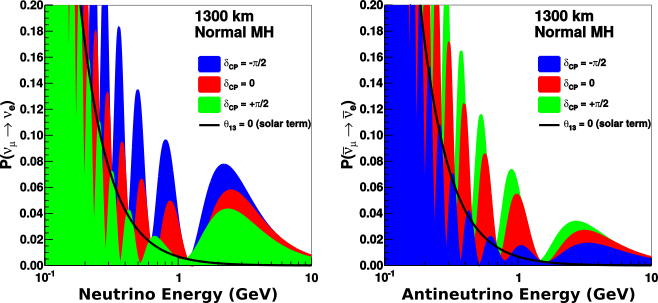
\includegraphics[width=\textwidth]{oscillation_CP.png} \\ \vspace{0.2cm}
                    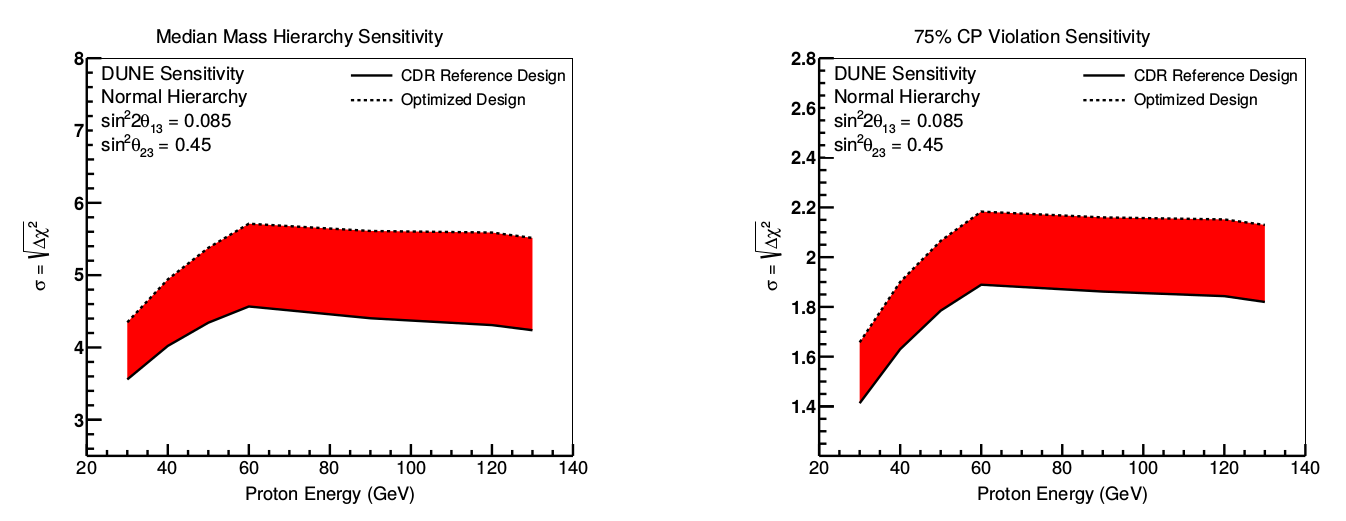
\includegraphics[width=0.95\textwidth]{sensitivities.png}\\
                    TDR de DU$\nu$E 2019
                \end{column}
                \begin{column}{0.4\textwidth}
                    \begin{scriptsize}
                        Pour atteindre ces sensibilités : \\
                    \end{scriptsize}
                    \begin{itemize}
                        \item Trajectographie 3D
                        \item Calorimétrie
                        \item PID
%                        \item Résolution en énergie $\leq$3\%
                    \end{itemize}
                \end{column}
            \end{columns}
        \end{scriptsize}
    \end{frame}

    \begin{frame}{DU$\nu$E : Deep Underground Neutrino Experiment}{Les 4 modules du détecteur lointain}
        \begin{scriptsize}
            \begin{columns}
                \begin{column}{0.55\textwidth}
                    \centering Le détecteur lointain\\
                    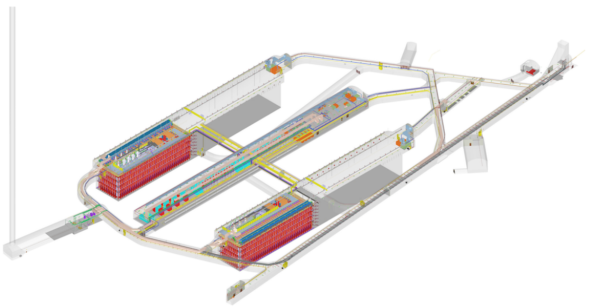
\includegraphics[width=0.8\textwidth]{./pictures/FD.png}\\
                    \centering Module simple phase\\
                    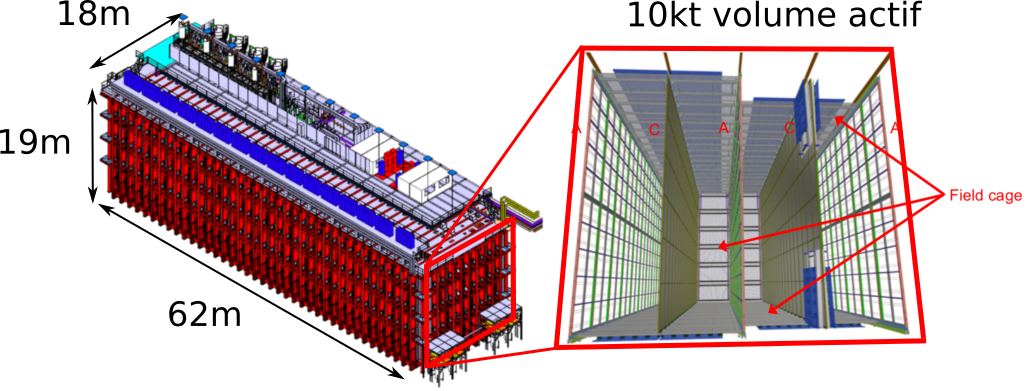
\includegraphics[width=\textwidth]{./pictures/module_SP.png}\\
                    \centering Module double phase (gauche) et intérieur de ProtoDU$\nu$E-DP (droite)\\
                    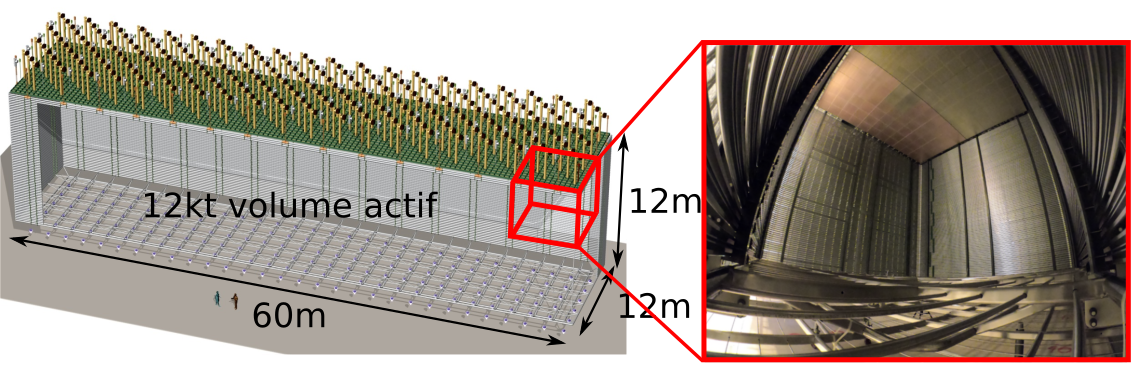
\includegraphics[width=0.9\textwidth]{./pictures/module_DP.png}
                \end{column}
                \begin{column}{0.45\textwidth}
                    \begin{itemize}
                        \item Détecteur lointain = $4\times\SI{10}{\kilo\tonne}$ modules de LArTPC
                        \item 2 Simple Phase, 1 Double phase, 1 à déterminer
                    \end{itemize}\vspace{0.4cm}
                    \textbf{Premier module SP} : été 2026.\\
                    \textbf{Premières données} : fin 2026\\
                    \textbf{Second module SP} : début 2028.\\\vspace{0.4cm}

                    $\Rightarrow$\textcolor{red}{\textbf{WA105/ProtoDU$\nu$E-DP}} est le prototype de la version \textcolor{red}{\textbf{Double Phase}} de la LArTPC.\\
                \end{column}
            \end{columns}
%            Timeline\\
        \end{scriptsize}
    \end{frame}
        
    \begin{frame}{La technologie LArTPC}{Chambres à Projection Temporelle à Argon Liquide}
       	\begin{scriptsize}
       			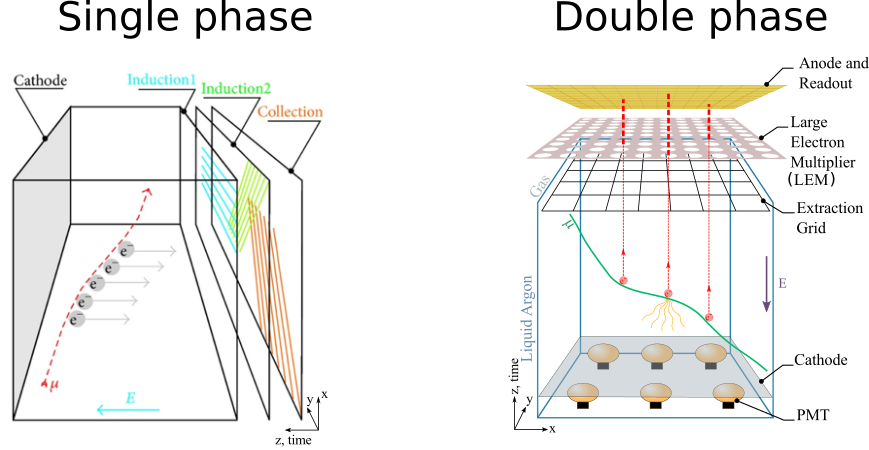
\includegraphics[width=0.9\textwidth]{tpcs.png}\\\vfill
       			\begin{columns}
       				\begin{column}{0.5\textwidth}
       					\begin{itemize}
       						\item Tout se passe dans l'argon liquide.
       						\item Reconstruction 3D des événements (précision millimétrique).
       						\item Mesure directe de l'énergie (précision $\sim\SI{100}{\kilo\electronvolt}$).
%       						\item Les premiers événements de protoDU$\nu$E-SP ont été vus l'an dernier.
       					\end{itemize}
       				\end{column}\hfill
       				\begin{column}{0.5\textwidth}
       					\begin{itemize}
       						\item \textcolor{red}{Amplification} des charges dans le gaz\\$\Rightarrow$ Meilleur ratio signal/bruit.
       						\item Plus grande distance de dérive, moins de canaux de lecture, meilleure résolution spatiale.
       						\item Premières données en septembre 2019.
       					\end{itemize}
       				\end{column}
       			\end{columns}
       	\end{scriptsize}
    \end{frame}
            
          \begin{frame}{L'argon liquide comme milieu de détection}
         	  \begin{scriptsize}
               	\begin{columns}
               		\begin{column}{0.6\textwidth}
               			\centering
               			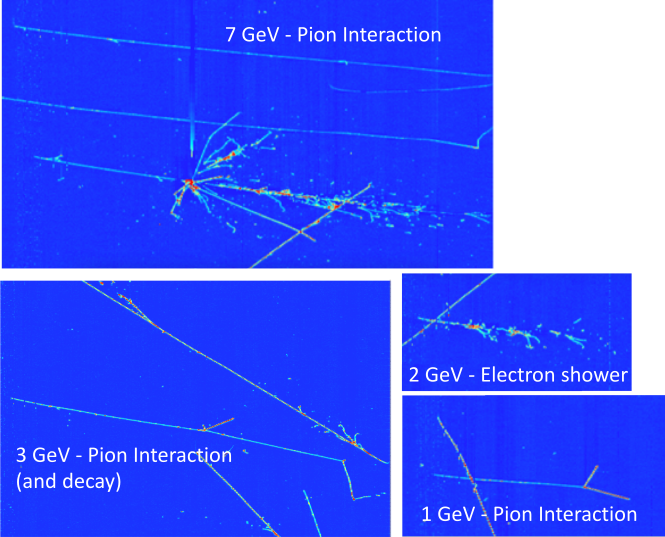
\includegraphics[width=\textwidth]{./pictures/SP_evt.png}\\
               			\flushleft
               			\begin{footnotesize}\textit{Événements dans protoDU$\nu$E-Simple Phase}\end{footnotesize}
               		\end{column}
               		\begin{column}{0.4\textwidth}
               			\begin{footnotesize}
               				\textbf{Pourquoi l'argon liquide?}
               			\end{footnotesize}
               			\begin{itemize}
               				\item Dense (\SI{1.4}{\gram\per\centi\meter^3}).
               				\item Peu cher et abondant.
               				(Bruit électronique $\sim \SI{1000}{e^-}$)
               				\item Gaz noble $\rightarrow$ ne piège pas les électrons.
               				\item Très bon trajectographe et calorimètre entièrement homogène.
               				\item Scintille au moment de l'ionisation $\rightarrow$ déclencheur et/ou $t_0$ \\ + transparent pour les photons  d'ionisation.
             				\item MIP $\rightarrow\sim\SI{60000}{e^-\per\centi\meter}$. \\
               			\end{itemize}
               			\begin{footnotesize}
           	    			\textbf{$\Rightarrow$ Chambre à bulle électronique.}
           	    		\end{footnotesize}
               		\end{column}
               	\end{columns}
         	  \end{scriptsize}
            \end{frame}
    
    \subsection{WA105}

    \begin{frame}{Le projet WA105/ProtoDU$\nu$E--DP}{WA105/\texorpdfstring{ProtoDU$\nu$E}{ProtoDUNE}--DP au CERN}
        \begin{scriptsize}
            \begin{columns}
                \begin{column}{0.75\textwidth}
                    \centering
                    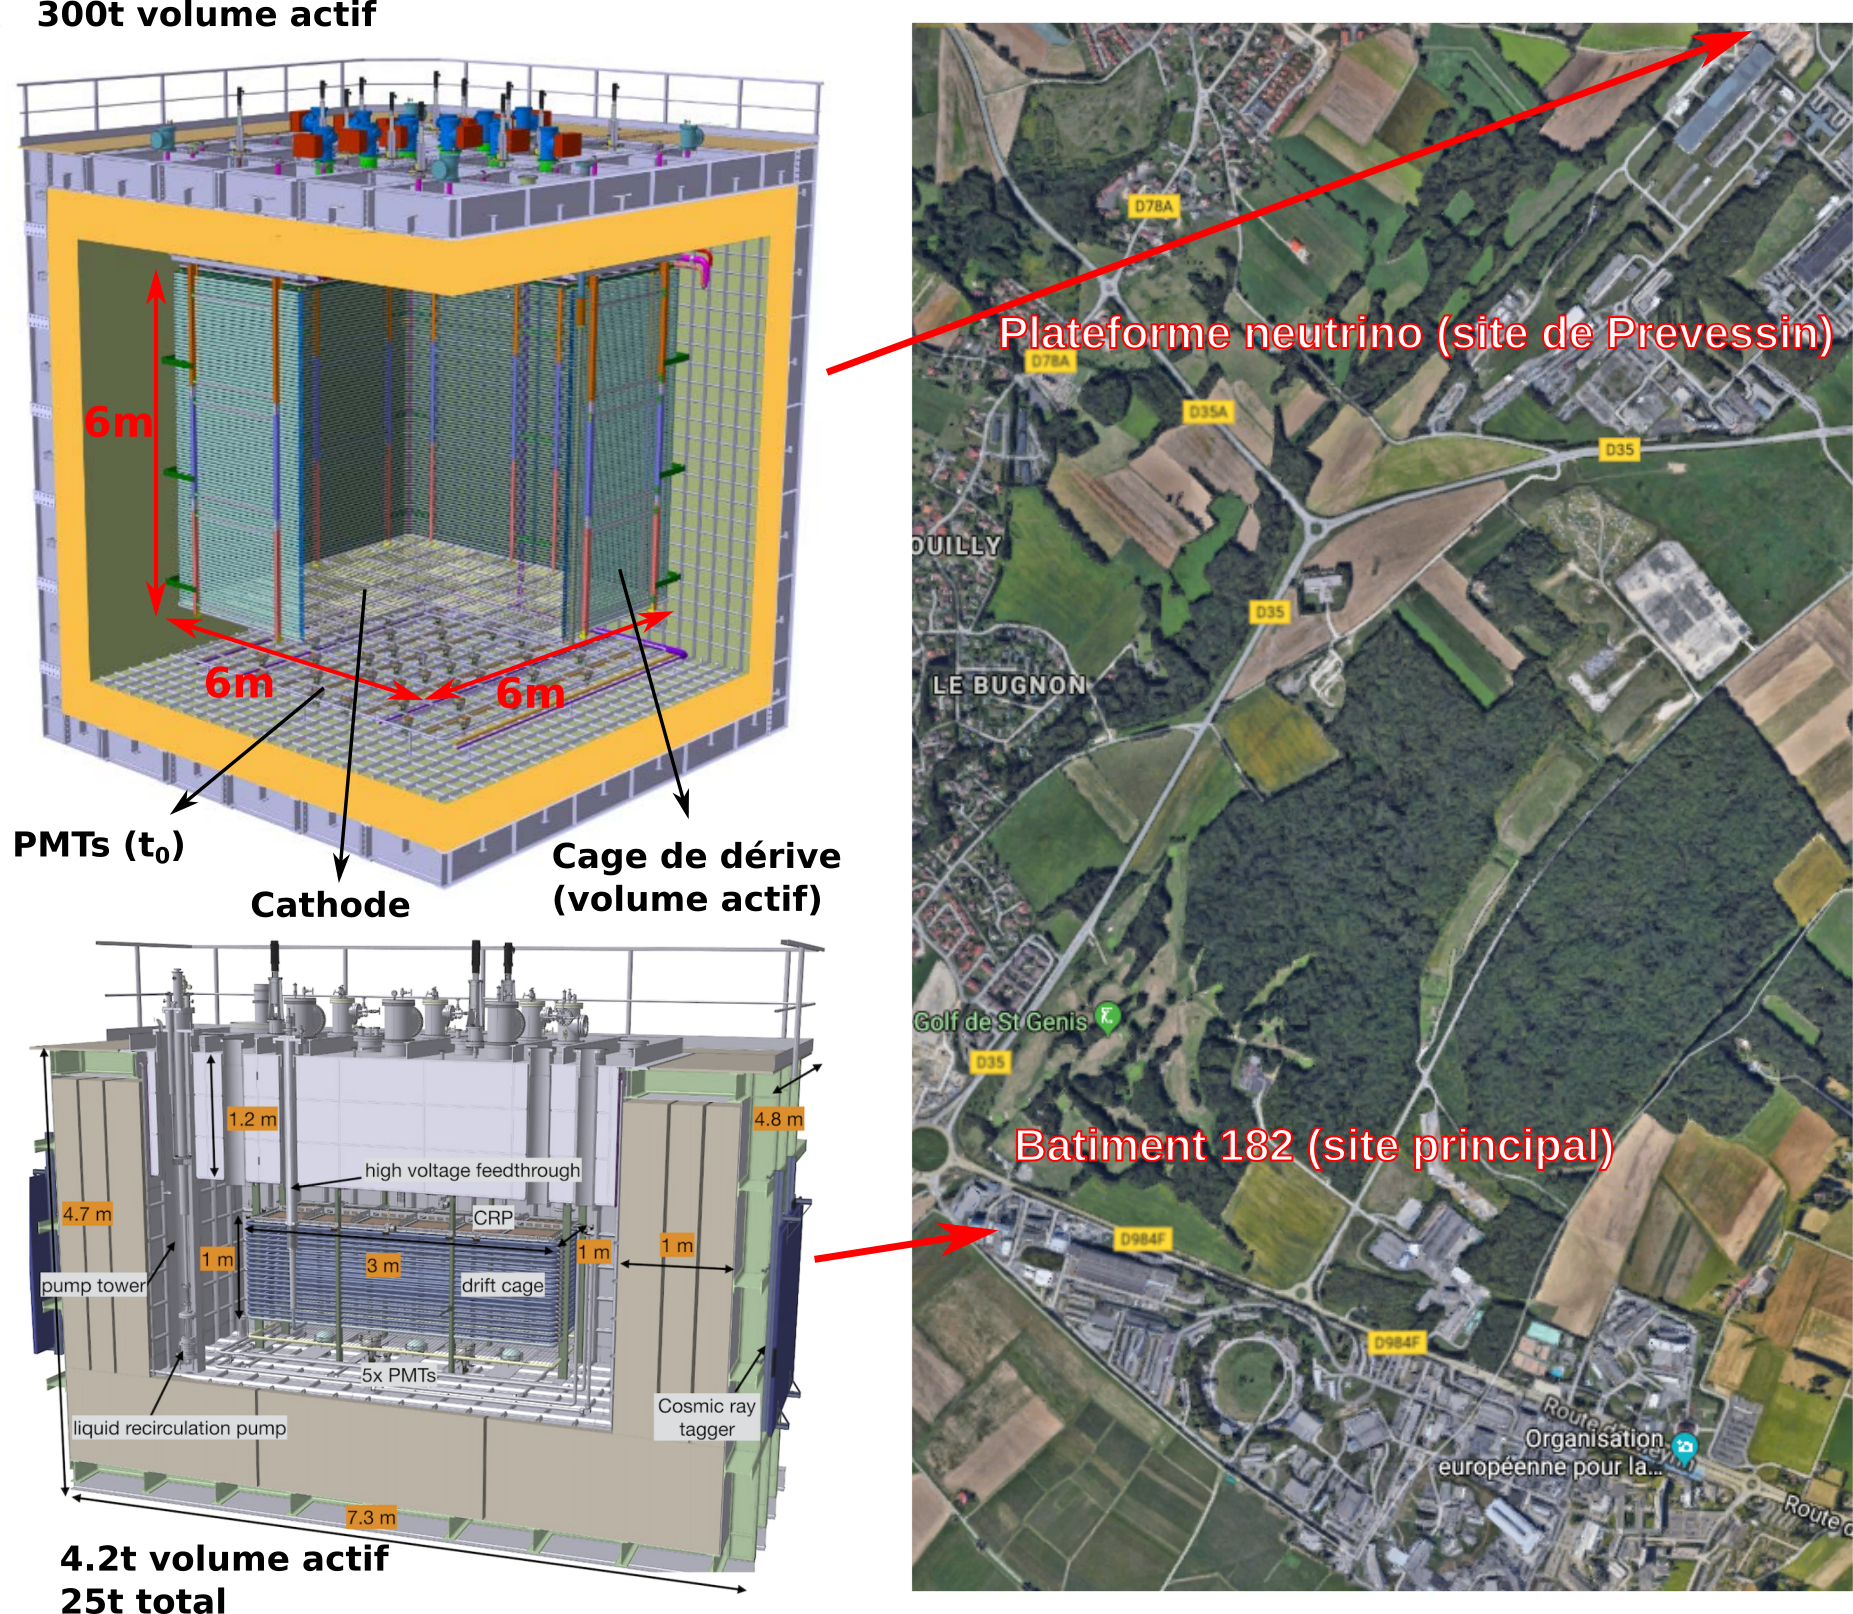
\includegraphics[width=\textwidth]{./pictures/wa105.png}
                \end{column}
                \begin{column}{0.25\textwidth}
                    \textbf{Démonstrateur de \SSS{} (\SI{300}{\tonne})}\\
                    \begin{itemize}
                        \item Teste DLArTPC à grande échelle
                        \item Directement extrapolable à DU$\nu$E
                        \item Mis en route en août 2019
                    \end{itemize}
                    \vspace{1cm}
                    \textbf{$+$ 1 premier prototype de \TOO{} (\SI{4}{\tonne})}\\
                    \begin{itemize}
                        \item Teste certains choix technologiques du \SSS{}
                        \item Opéré en 2017
                    \end{itemize}
                \end{column}
            \end{columns}
        \end{scriptsize}
    \end{frame}

    \begin{frame}{La technologie DLArTPC}
        \centering
       	\vspace{-0.5cm}\hspace{-0.4cm}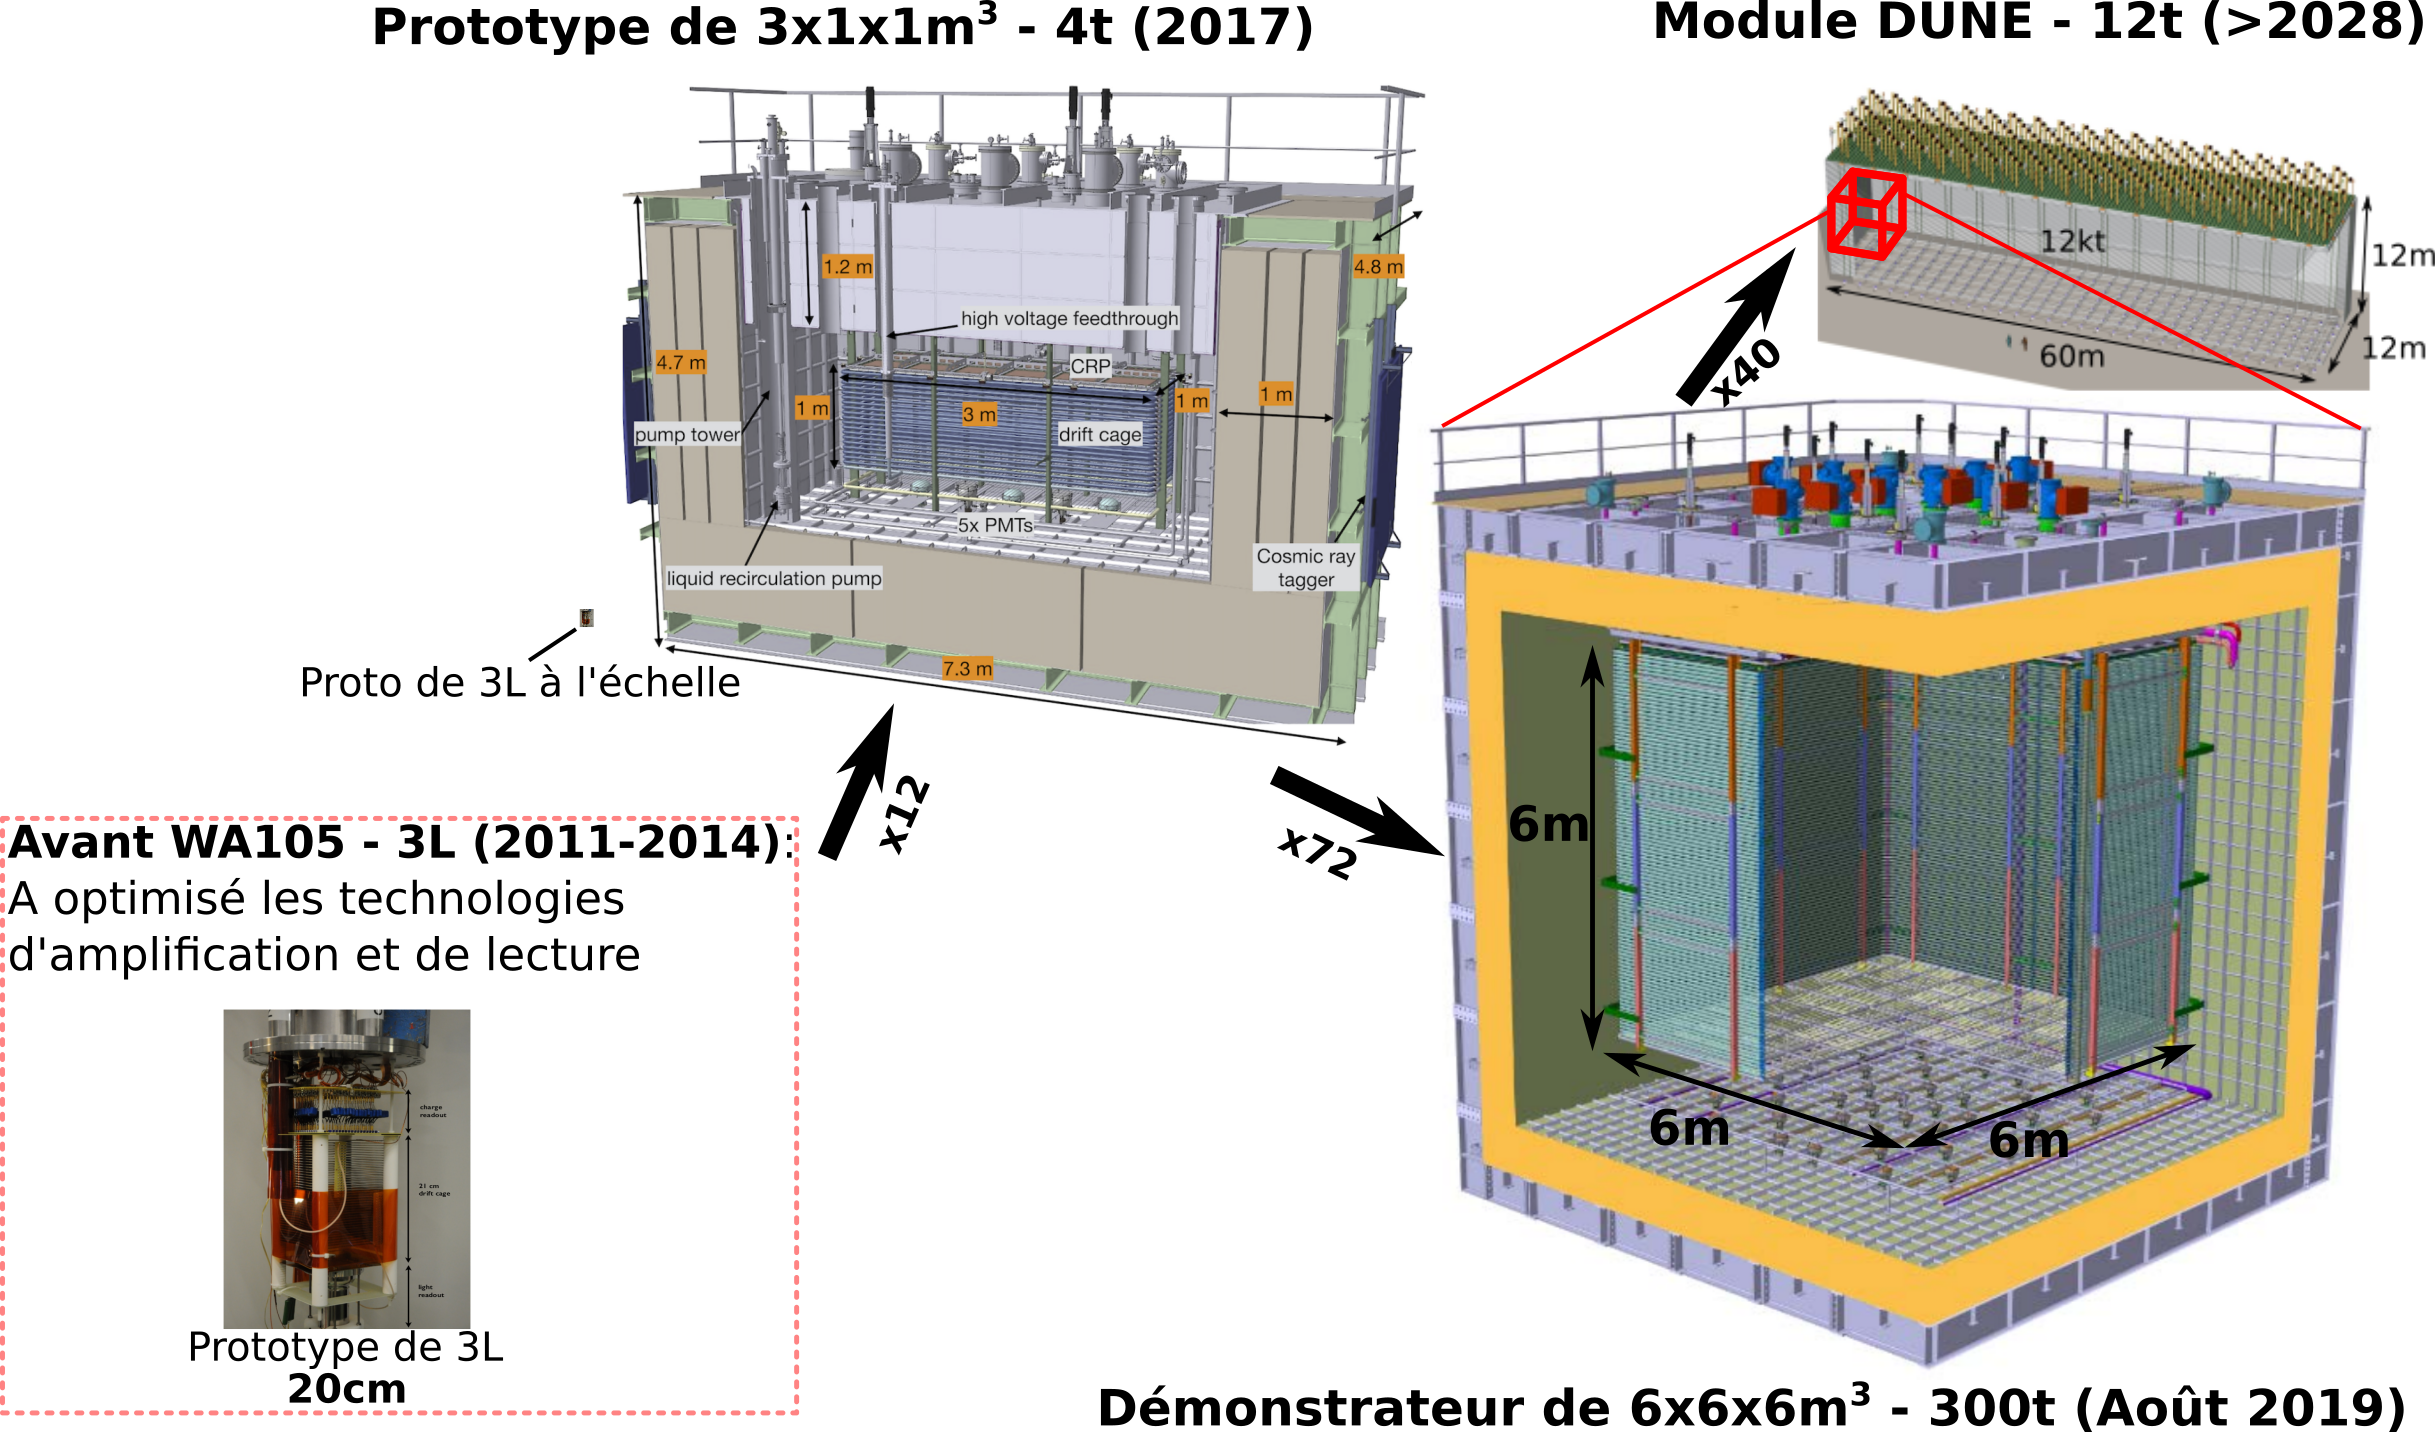
\includegraphics[width=1.03\linewidth]{wa105_scales.png}
    \end{frame}

%  {
%    	\setlength\pdfpagewidth{12.8cm}%
%    	\setlength\pdfpageheight{9.15cm}%
%    	\usebackgroundtemplate{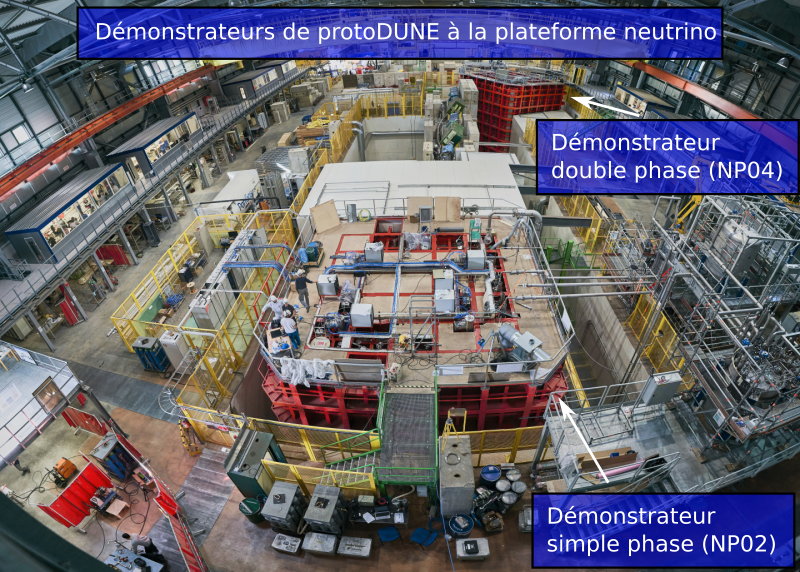
\includegraphics[width=\paperwidth]{nu_platform.png}}
%    	\begin{frame}[plain]
%    	\end{frame}
%    }
    
    \section[Tests des LEMs]{Tests et mesures des détecteurs LEMs du démonstrateur de \SI{300}{\tonne}}

    {
    	\usebackgroundtemplate{
\includegraphics[width=\paperwidth]{./pictures/1.pdf}}
        \begin{specialframe}
            \vspace{2cm}\hspace*{-1.8cm}\parbox[t]{\textwidth}{
                \begin{center}
                    \begin{Huge}
                            \textcolor{pheniics_purple}{\textbf{\insertsection}}
                    \end{Huge}
                \end{center}
            }
        \end{specialframe}
    }

    \begin{frame}{Le démonstrateur de \SSS{}}
    	\begin{scriptsize}
                \centering
    			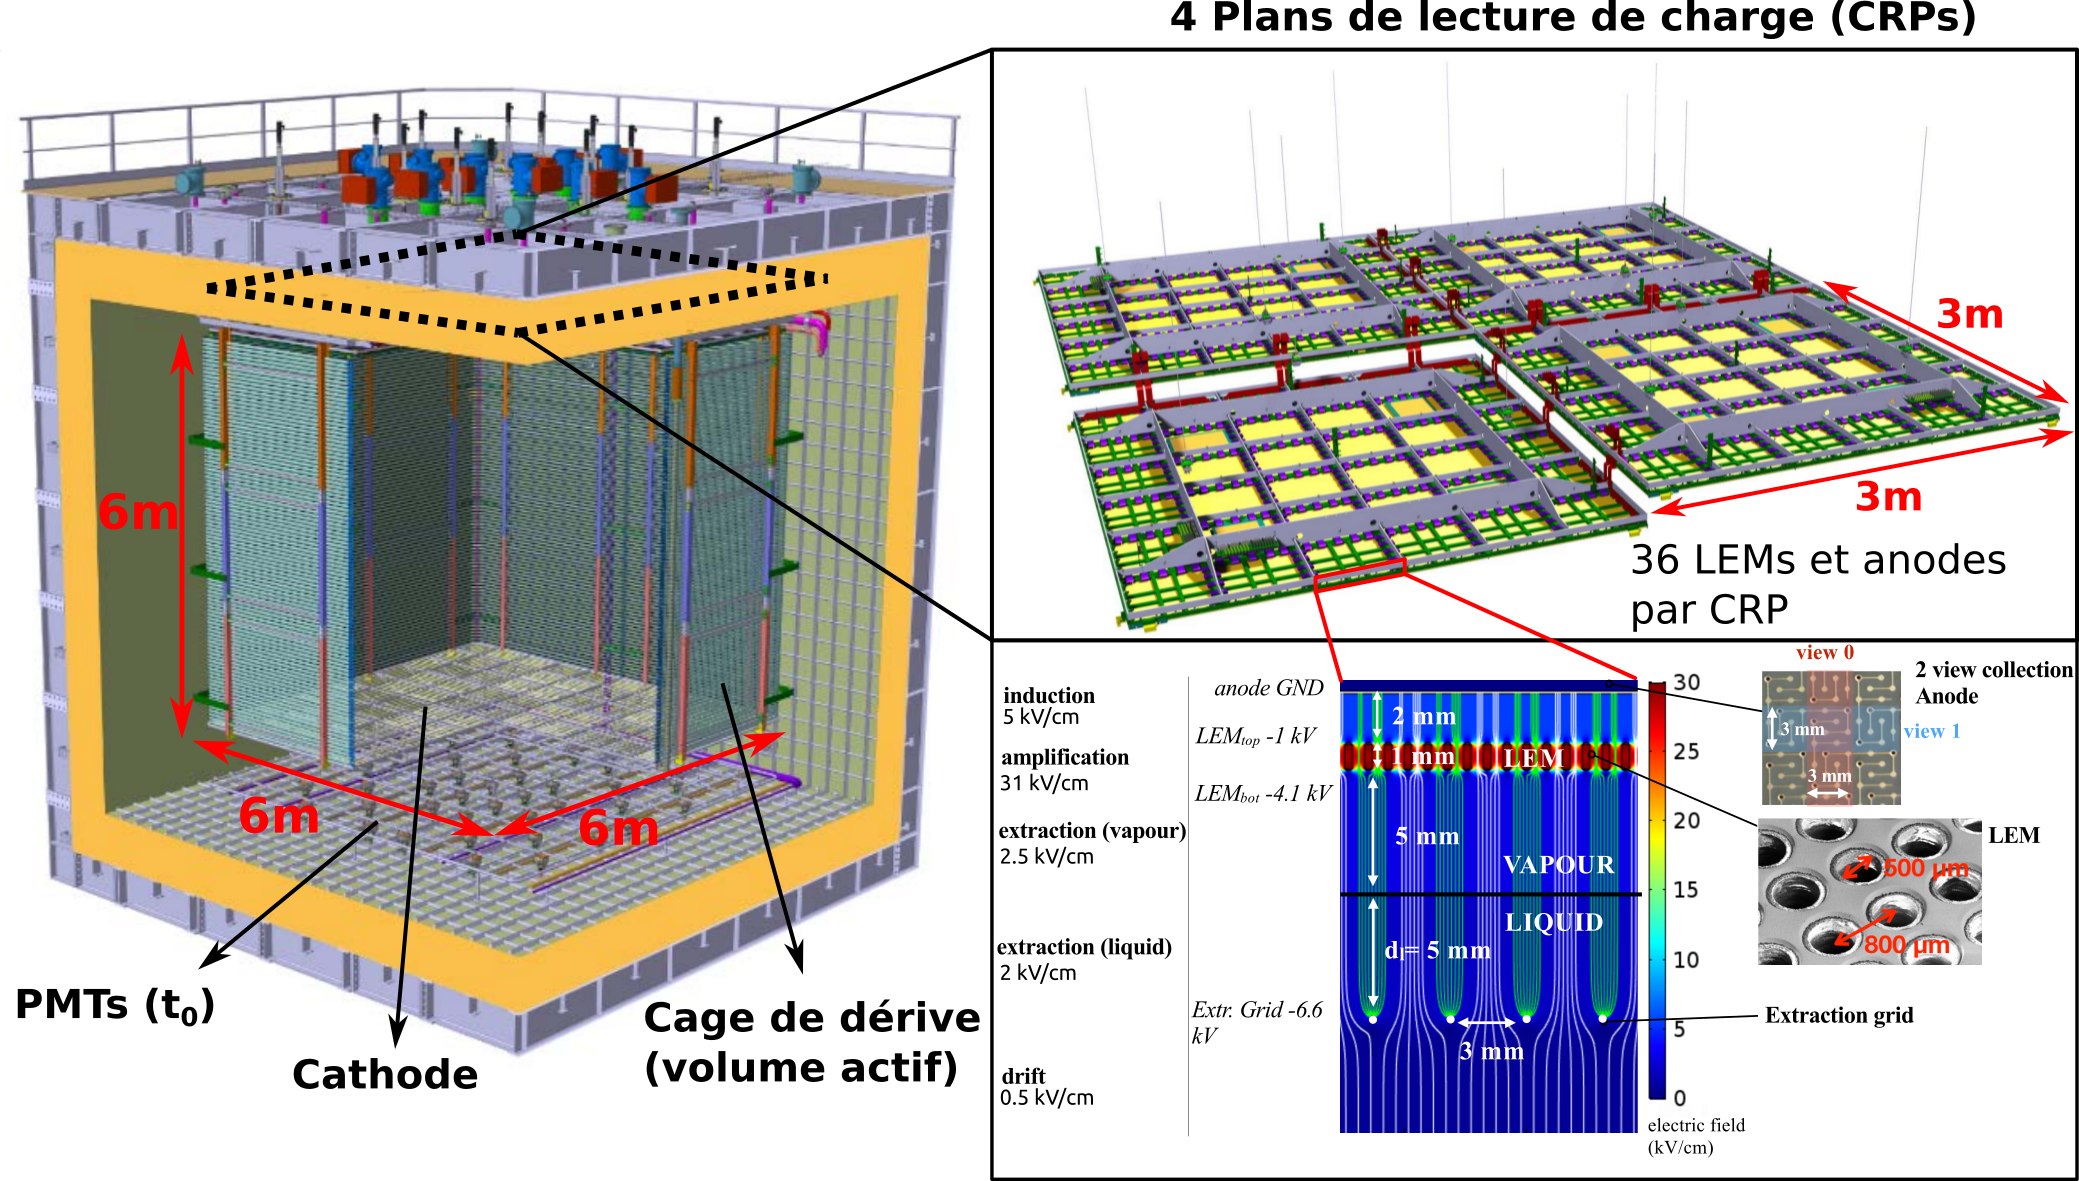
\includegraphics[width=0.9\textwidth]{666_full.png}\\
    			\vfill
    			\textbf{Nouvelle technologie : principaux défis :}\\
    			\begin{minipage}{0.32\textwidth}
    				\begin{itemize}
    					\item \textcolor{red}{But: Gain $\geq 20$} \\(S/B $\geq 200$ pour une MIP)
    					\item \textcolor{red}{Stabilité (plusieurs années)}
    				\end{itemize}
    			\end{minipage}\hfill
    			\begin{minipage}{0.32\textwidth}
    				\begin{itemize}
    					\item Impuretés: 0.1\;ppb
    					\item \SI{6}{\meter} de dérive : \SI{500}{\volt\per\centi\meter} $\Rightarrow$ Cathode à \SI{300}{\kilo\volt}
    				\end{itemize}
	    		\end{minipage}\hfill
	    		\begin{minipage}{0.32\textwidth}
	    			\begin{itemize}
    					\item[\danger] Effet de charge d'espace (pas dans DU$\nu$E)
	    			\end{itemize}
	    		\end{minipage}
    	\end{scriptsize} 
    \end{frame}

    \begin{frame}{Le sandwich LEM-anode}
	   		\begin{minipage}{0.48\textwidth}
	   			\begin{scriptsize}
		   			\textbf{Gain effectif:}\\
		   		\end{scriptsize}
	   			$G_{eff} = \mathcal{T}e^{A\rho d e^{-B\rho d/V}}$\\
	   			\begin{scriptsize}
	    			\begin{itemize}
	    				\item $\mathcal{T}$: Transparence au électrons du sandwich LEM-anode.
	    				\item $A,B$: coefficients, dépendent du gaz.
	    				\item $d$: distance d'amplification (\SI{1}{\milli\meter}).
	    				\item $V$: tension d'amplification ($\sim$\SI{3}{\kilo\volt}).
	    				\item $\rho$: densité du gaz ($\propto P/T$).
	    			\end{itemize}
	    		\end{scriptsize} 
	   			\vfill
                \centering
				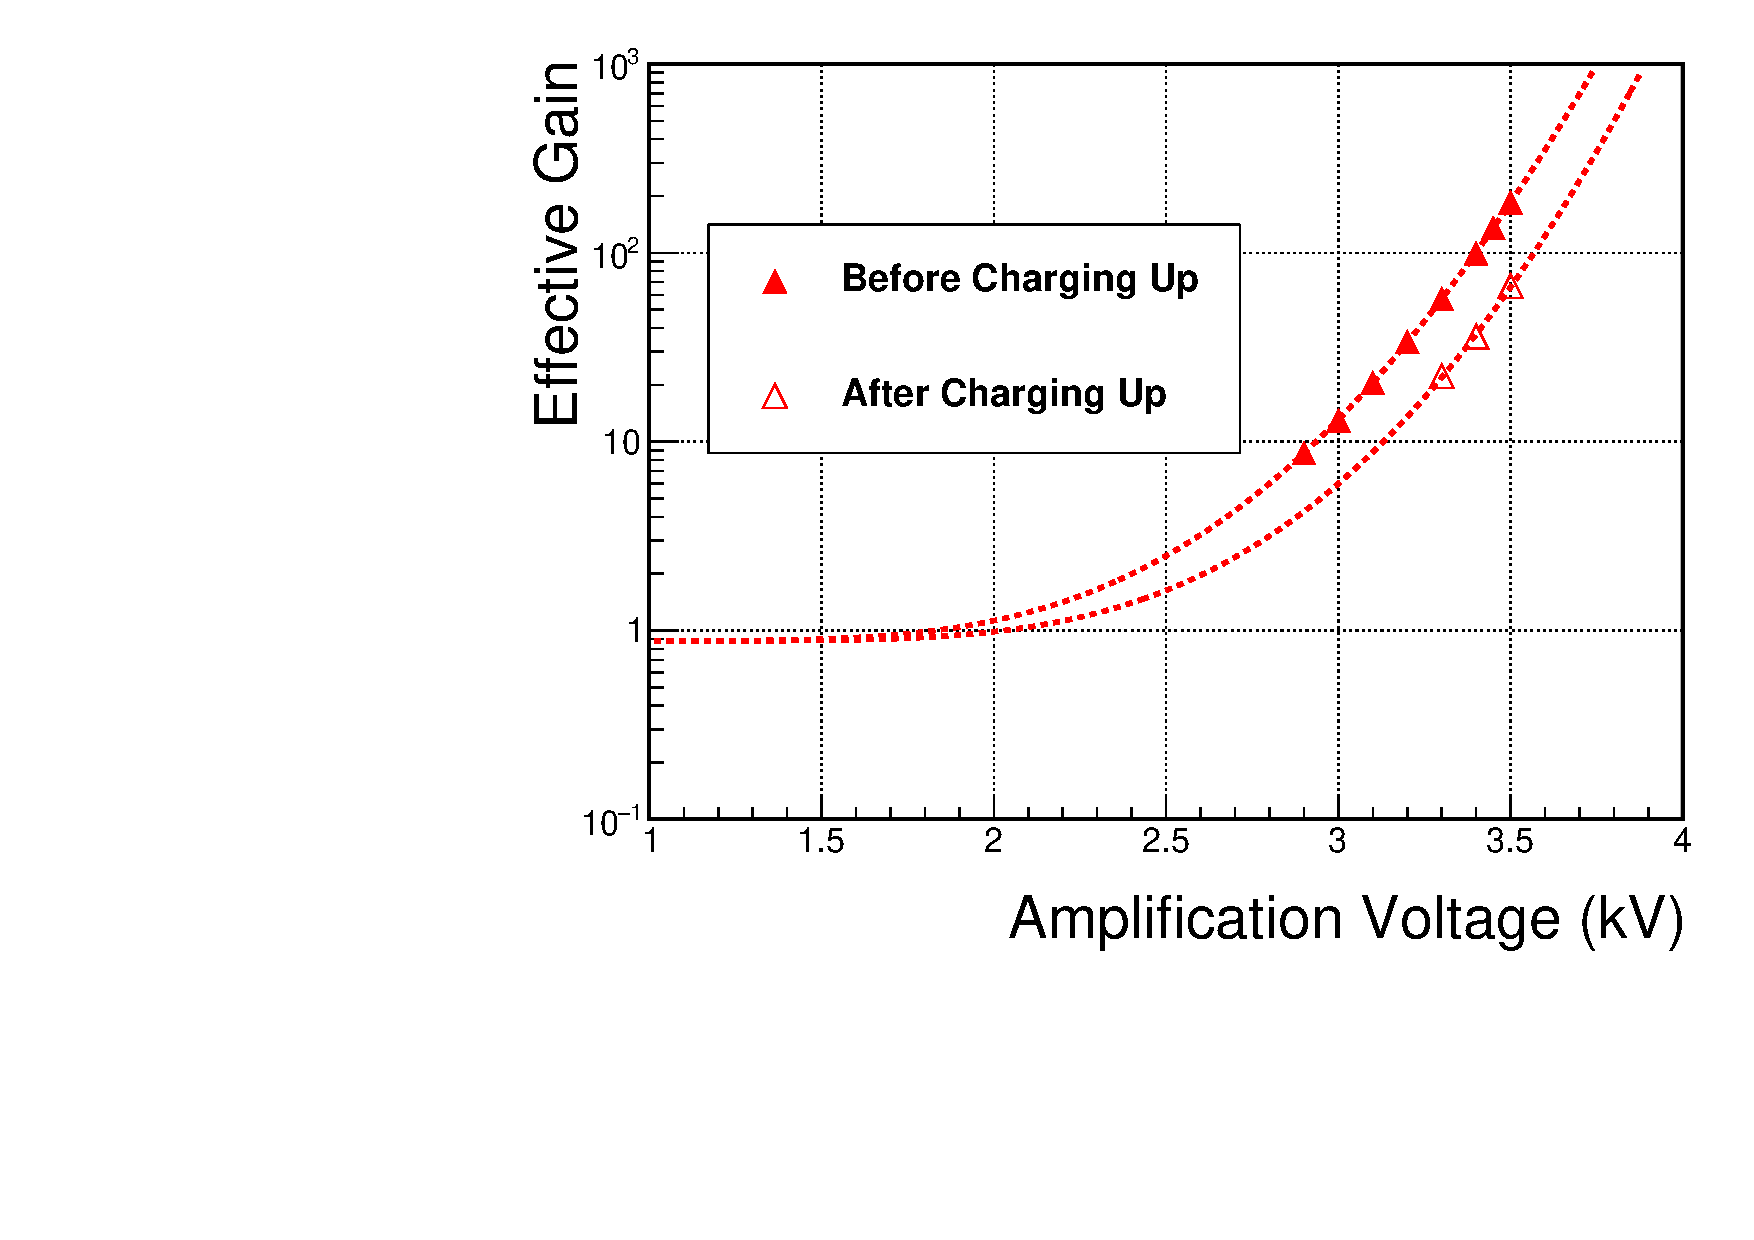
\includegraphics[width=0.8\textwidth]{gain_3L.pdf}\\\tiny{C. Cantini et al., 2014, doi : 10.1088/1748-0221/10/03/P03017}
	   		\end{minipage}\hfill
	   		\begin{minipage}{0.48\textwidth}
	   			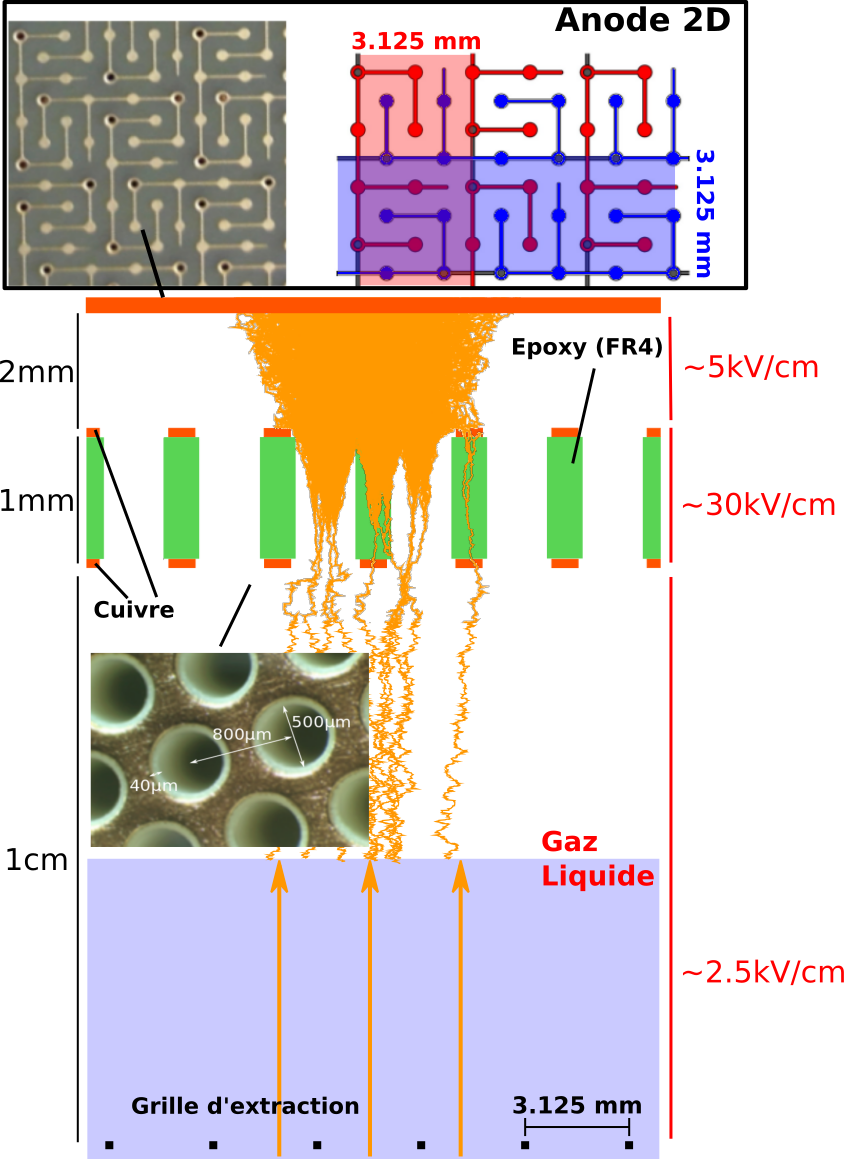
\includegraphics[width=\textwidth]{lem_anode.png}
	   		\end{minipage}
    \end{frame}
    
    \begin{frame}{Le charging up}
        \begin{scriptsize}
            \begin{columns}
      			\begin{column}{0.5\textwidth}
          			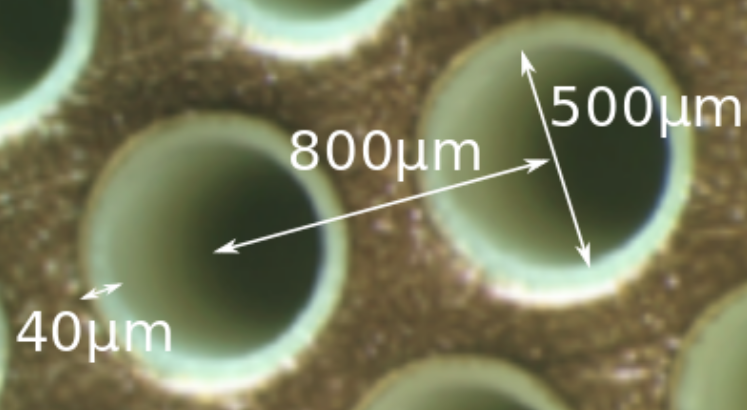
\includegraphics[width=\textwidth]{RIM.png}\\\vspace{1cm}
      				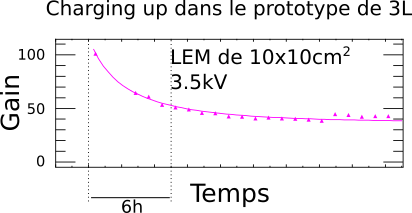
\includegraphics[width=\textwidth]{3L_charging_up.png}\\
      			\end{column}\hfill
      			\begin{column}{0.5\textwidth}
      				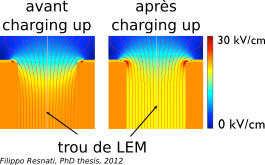
\includegraphics[width=\textwidth]{CU.png}\\\vspace{1cm}
          			\textbf{RIM autour des trous :}
      				\begin{itemize}
      					\item[$\Rightarrow$] Lignes de champ traversent le FR4\\
      					\item[$\Rightarrow$] L'accumulation d'électron \textcolor{blue}{déforme et atténue} le champ
%    					\item Le temps de charging up time dépend de la tension dans le LEM et du taux de dépôt de charge.
      				\end{itemize}
      				Charging up: \textcolor{red}{$G_{eff}(t)$ décroît} jusqu'à un plateau ($\sim$ quelques jours).
      			\end{column}
      		\end{columns}
        \end{scriptsize}
    \end{frame}

    \begin{frame}{La mission de l'Irfu}
        \centering \textbf{\textcolor{red}{Mission de l'Irfu}: }Production, test et caractérisation des LEMs et anodes de 2 des 4 CRPs.\\\vfill
    	\begin{scriptsize}
        	\begin{columns}
            	\begin{column}{0.5\textwidth}
                	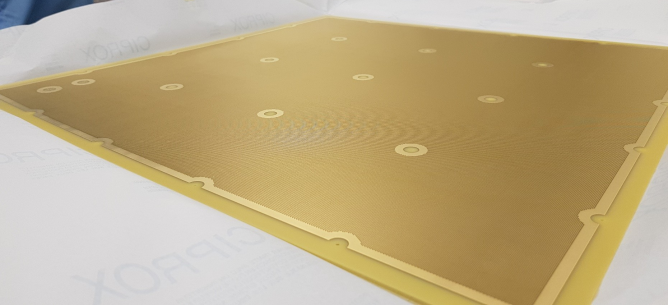
\includegraphics[width=\textwidth]{./pictures/LEM.png}\\
                   	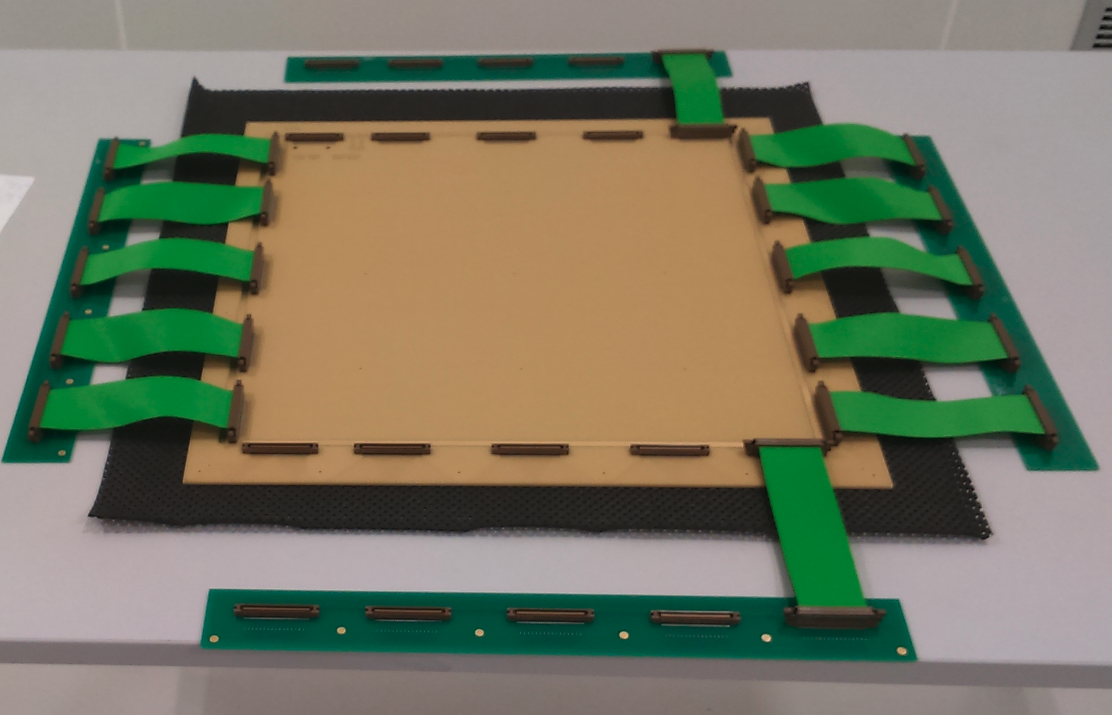
\includegraphics[width=\textwidth]{anode_carde.png}
            	\end{column}
       	        \begin{column}{0.5\textwidth}
           	        \textbf{Tenue en tension?\\
           	        Gain?\\
           	        Uniformité de l'épaisseur des LEMs?\\
           	        Continuité des pistes des anodes?\\}\vspace{0.3cm}
           	        \begin{itemize}
               	        \item Réalisation de l'infrastructure nécessaire aux tests des LEMs et anodes
               	        \item LEMs produit par ELTOS sur la base du design testé dans le prototype de \threeL{} par ETHZ (CFR-34, été 2017)
               	        \item Modification du design afin d'atteindre une meilleure tenue en tension (CFR-35, Janvier--Octobre 2018)
               	        \item Instrumentation de 2 CRPs sur 4
           	        \end{itemize}
       	        \end{column}
        	\end{columns}
   		\end{scriptsize}
    \end{frame}

    \begin{frame}{Préparation des LEMs}
    	\begin{scriptsize}
    		\begin{center}
		    	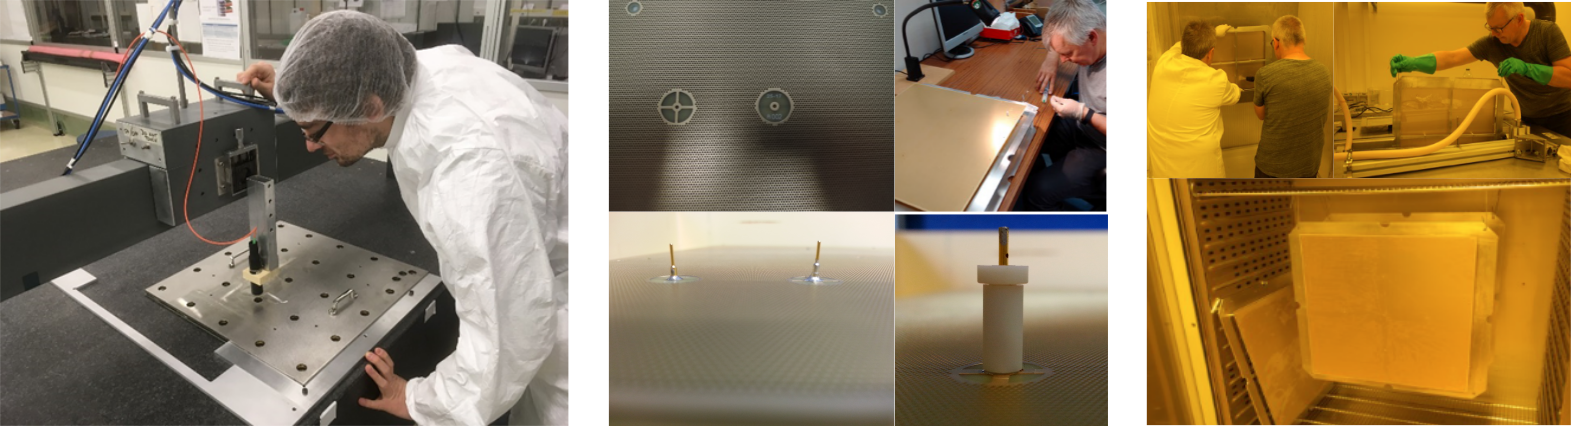
\includegraphics[width=\textwidth]{pretest.png}
	    	\end{center}
	    	\begin{columns}
	    		\begin{column}{0.5\textwidth}
	    			\begin{itemize}
	    				\item ELTOS mesure l'épaisseur des LEMs et s'assure du respect du cahier des charges
	    			\end{itemize}
	    		\end{column}\hfill
	    		\begin{column}{0.5\textwidth}
	    			\textbf{\hspace{0.3cm}Au CEA (DEDIP)}:
	    			\begin{itemize}
	    				\item Contrôle de l'uniformité de l'épaisseur.
	    				\item Soudure et collage.
	    				\item Nettoyage, polymérisation, séchage.
	    			\end{itemize}
	    		\end{column}
	    	\end{columns}
	    \end{scriptsize}
	    \vspace{0.5cm}
        $\Rightarrow$ LEM prêts pour les tests hautes tensions et mesures de gain!
    \end{frame}

    \subsection[Épaisseur]{Mesure de l'épaisseur des LEMs}

     \begin{frame}{Mesure de l'épaisseur des LEMs}{Méthode expérimentale}
    	\begin{scriptsize}
    		\begin{columns}
    			\begin{column}{0.5\textwidth}
    				\begin{center}
    					$G _{eff}= \mathcal{T}e^{A\rho \textcolor{red}{d} e^{-B\rho \textcolor{red}{d}/V}}$\\
    				\end{center}
    				$\textcolor{red}{d}$: \textcolor{red}{épaisseur du LEM}.\\
    				$\Rightarrow$ Impact exponentiel sur le gain.\\
    				$\Rightarrow$ Nécessaire de connaître les fluctuations de cette épaisseur pour \textcolor{red}{vérifier l'uniformité du gain}.\\
    				\vfill
    				\centering 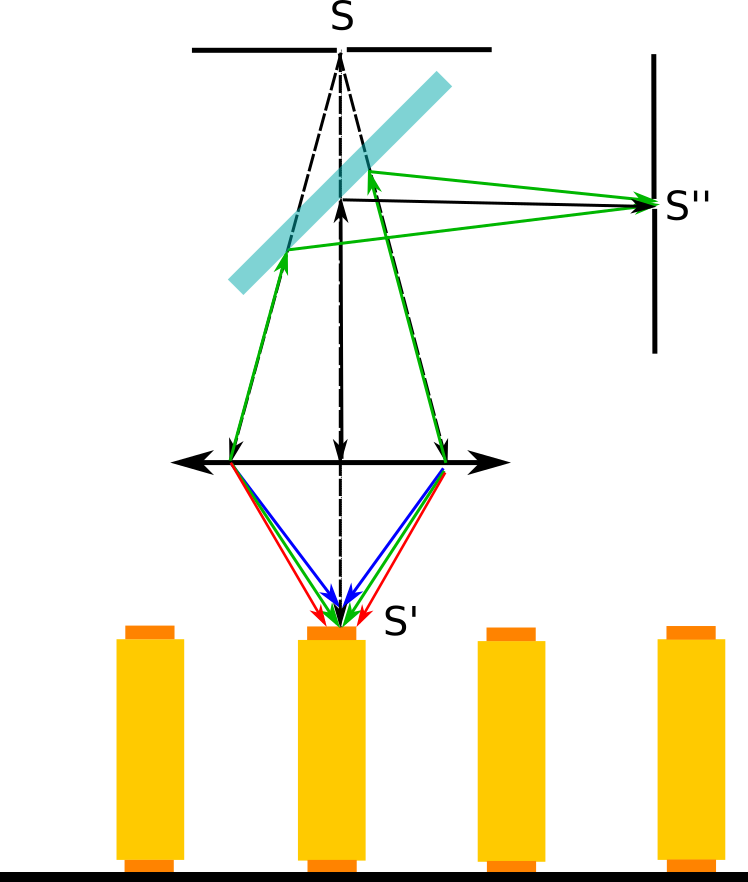
\includegraphics[height=0.6\textheight]{CCI.png}\\\vfill
    			\end{column}
    			\hfill
    			\begin{column}{0.5\textwidth}
    				\begin{itemize}
    					\item Imagerie Chromatique Confocale.
    					\item Mesure l'épaisseur des 72 LEMs du \SSS{}.
    					\item Création d'un script Python pour l'analyse des résultats.
    				\end{itemize}
    				\centering 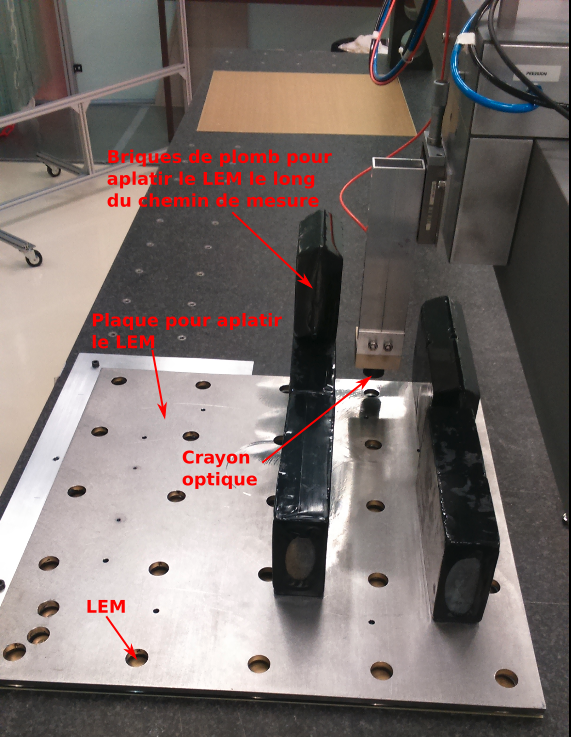
\includegraphics[height=0.6\textheight]{./pictures/plate_and_bricks.png}\\
    			\end{column}
    		\end{columns}
    	\end{scriptsize}
    \end{frame}

    \begin{frame}{Mesure de l'épaisseur des LEMs}{Résultats}
    	\begin{scriptsize}
    		\begin{columns}
    			\begin{column}{0.48\textwidth}
    				\centering
    				Épaisseur dans un trou de mesure\\
    				\centering
    				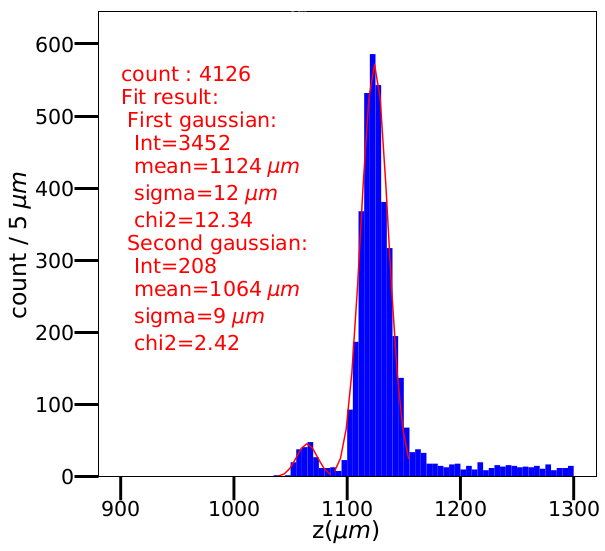
\includegraphics[width=0.7\textwidth]{distri_1_trou_lem.png}\\
    				\vspace{0.15cm}
    				\centering
    				Épaisseur moyenne (36 LEMs)\\
    				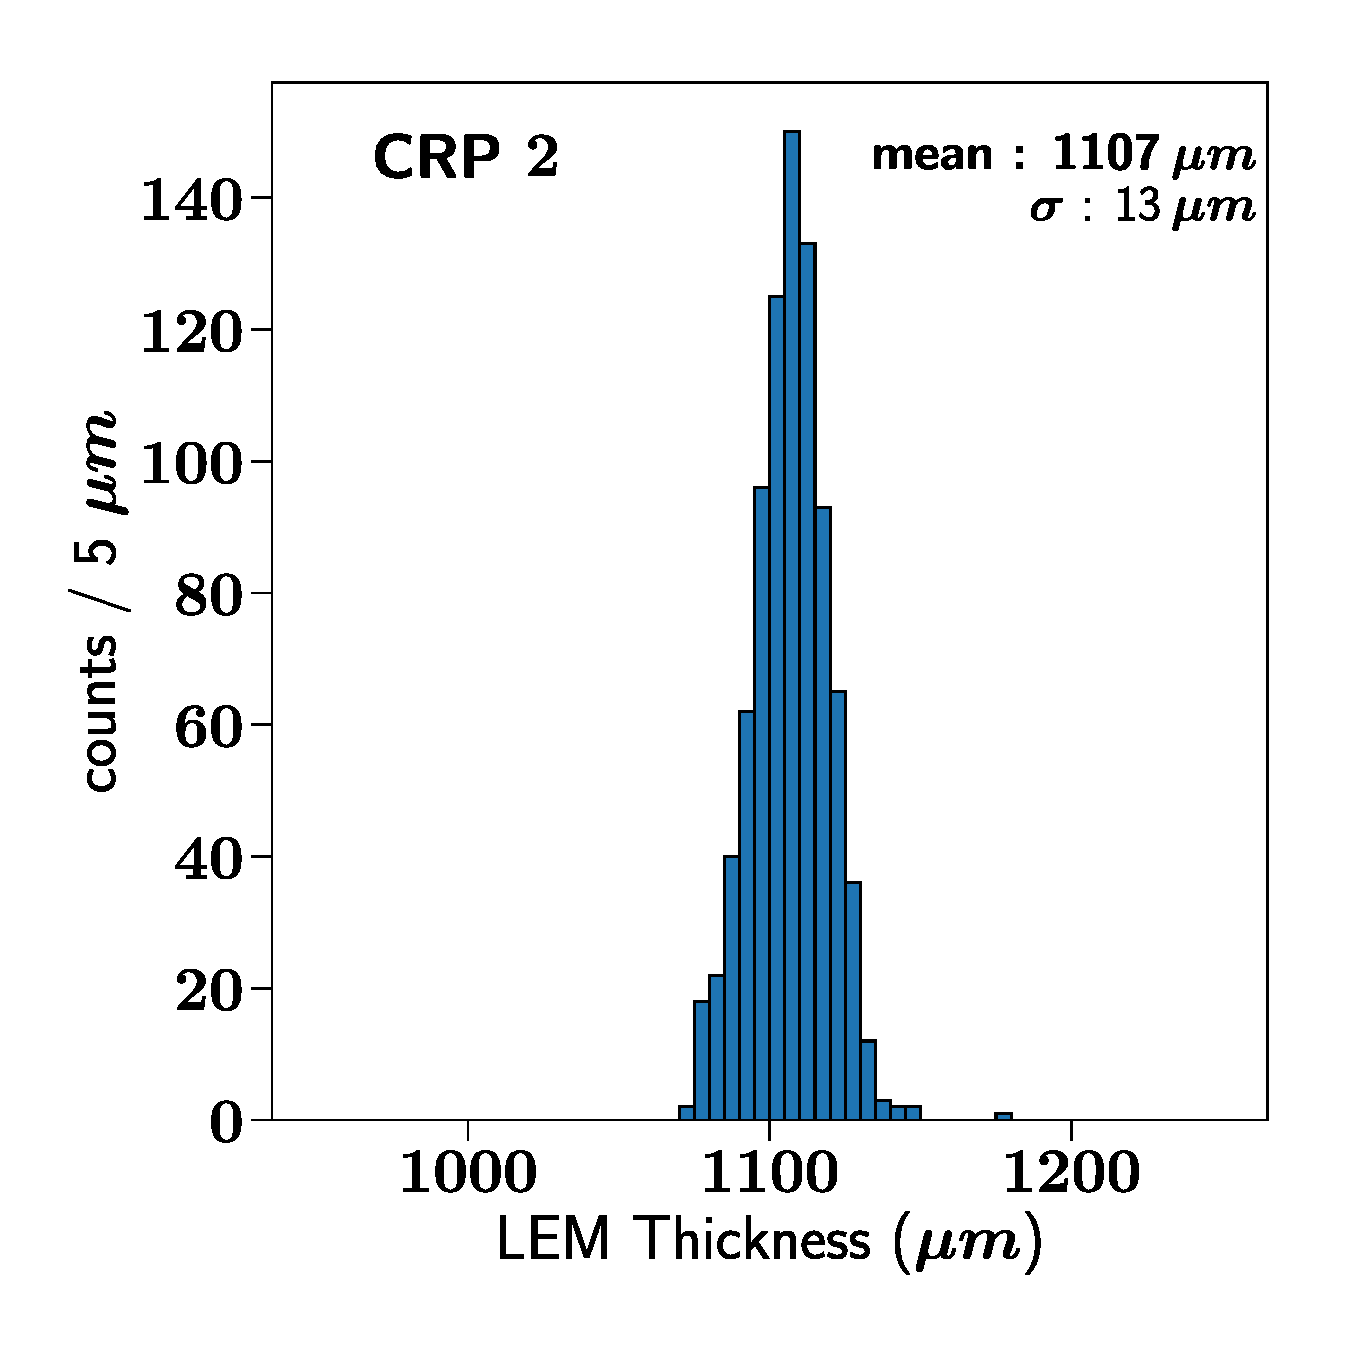
\includegraphics[width=0.7\textwidth]{LEM_sum_all_histo_CERN.pdf}
    			\end{column}
    			\hfill
    			\begin{column}{0.48\textwidth}
    				\centering
    				Uniformité de l'épaisseur dans 1 LEM\\
    				\centering
    				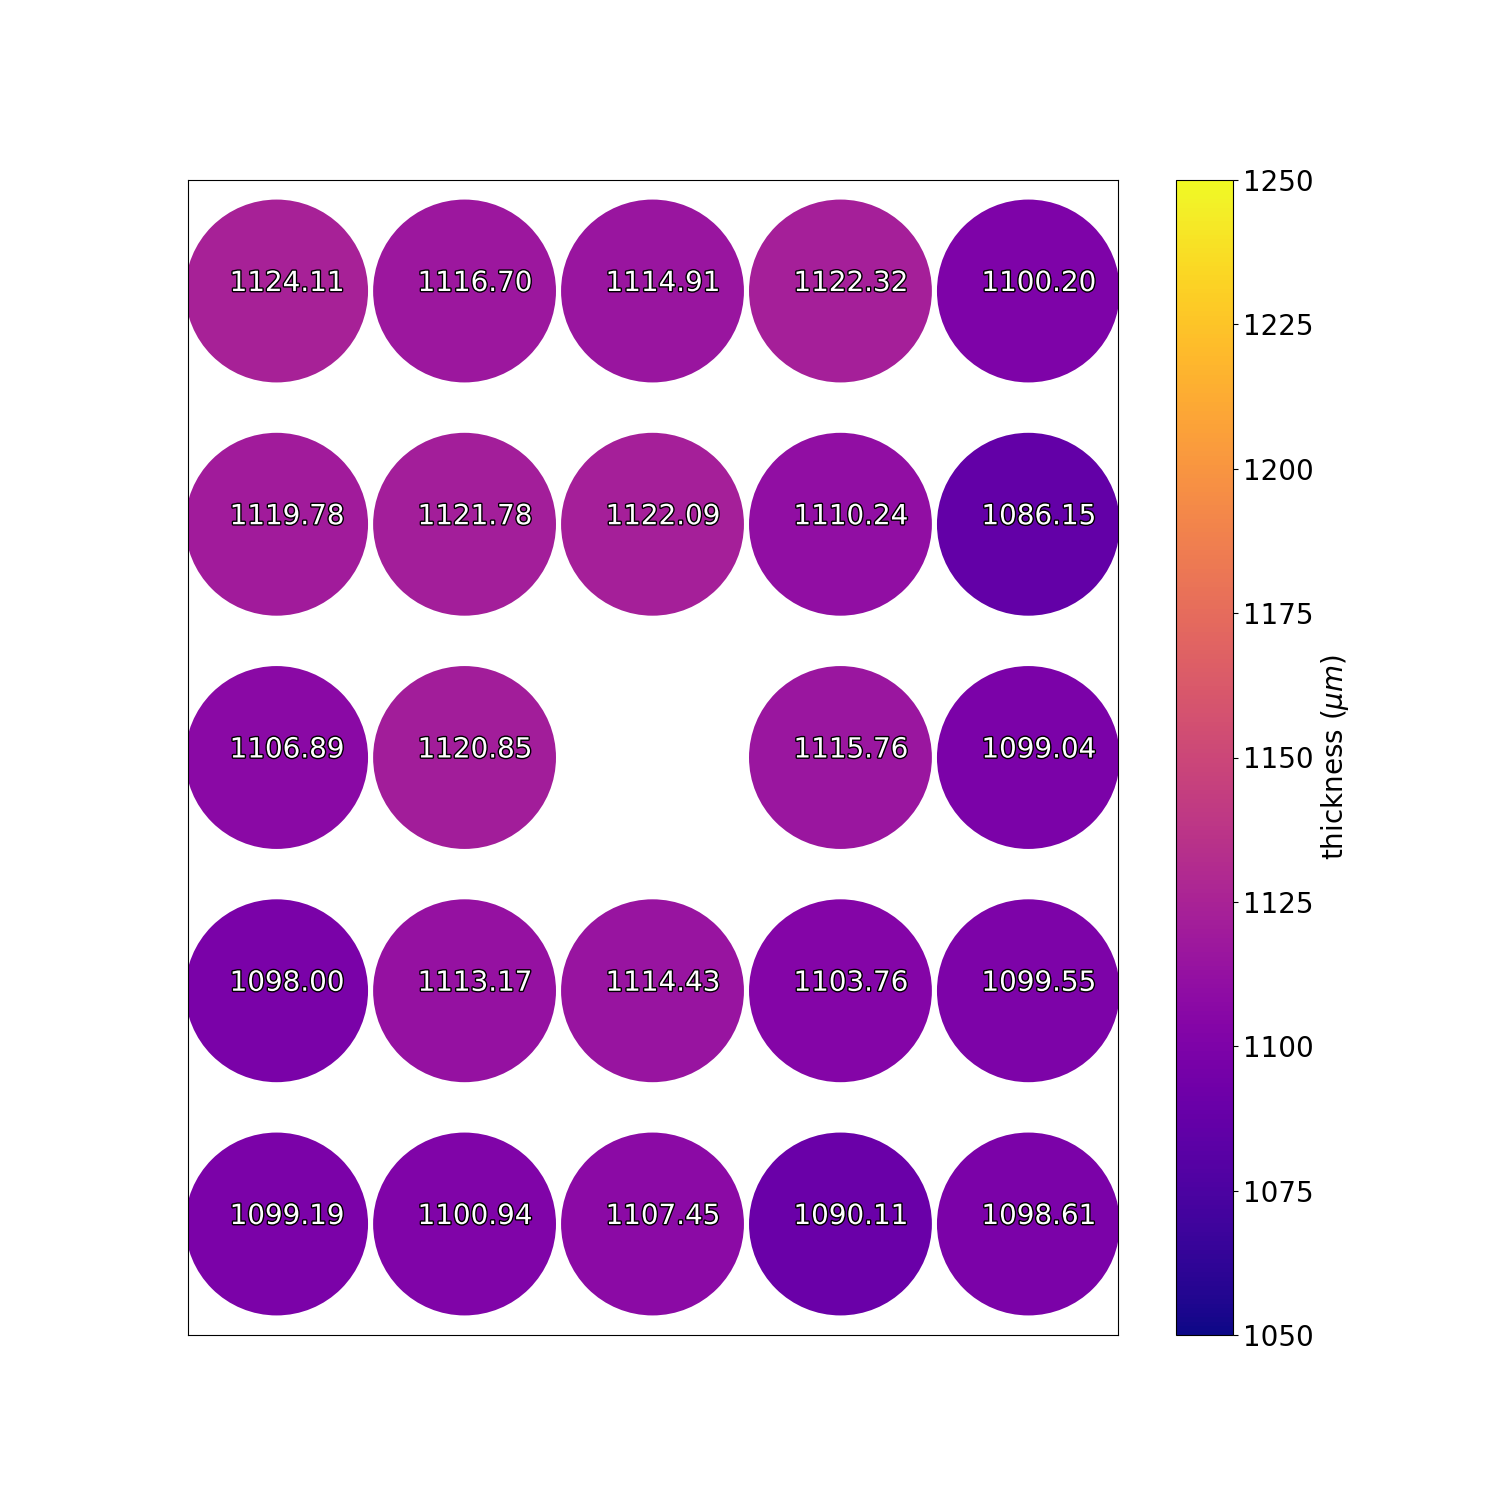
\includegraphics[width=0.6\textwidth]{2D_LEM_thickness_distri.png}\\
    				\vspace{0.15cm}
    				\centering
    				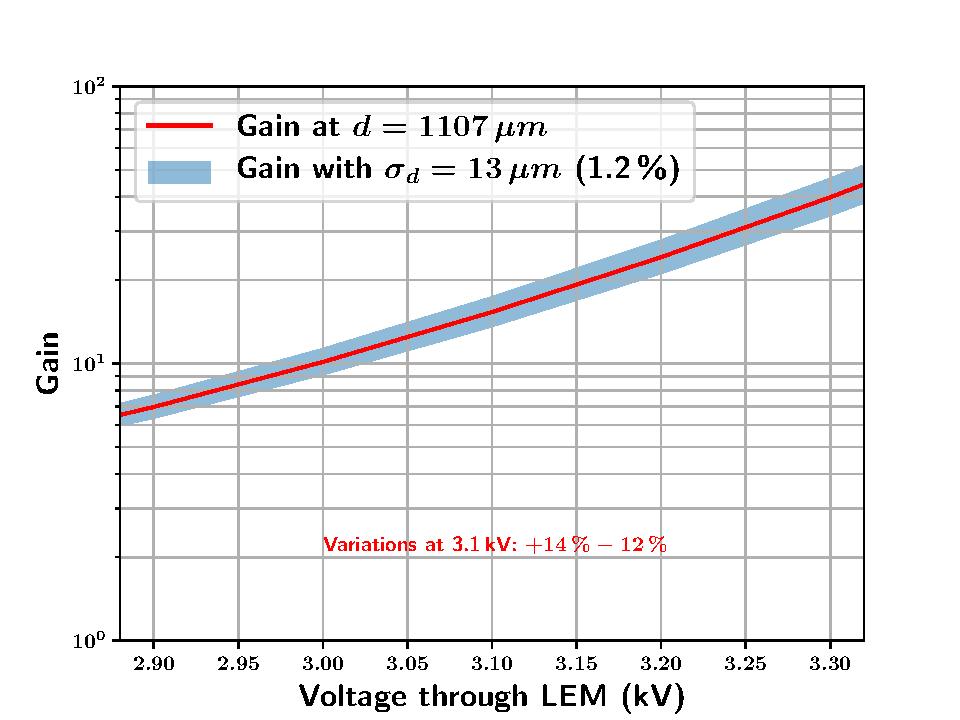
\includegraphics[width=\textwidth]{measured_gain_fluctuations.pdf}
    			\end{column}
    		\end{columns}
    	\end{scriptsize}
    \end{frame}

%  \begin{frame}{frame title}{frame subtitle}
%      \begin{block}{LEMs}
%        \begin{columns}
%          \column{.5\textwidth} \hspace{0.5cm}
%          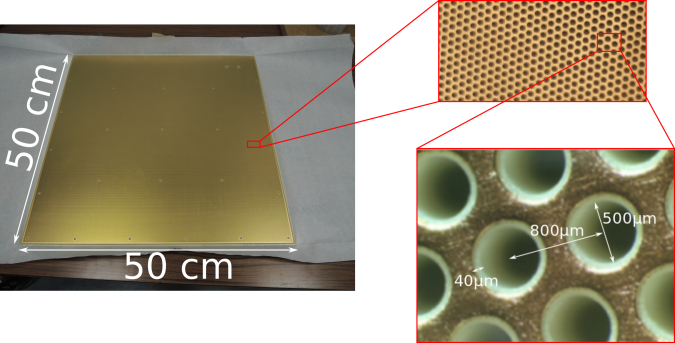
\includegraphics[width=0.7\textwidth]{LEM_zoom.png} 
%          \column{.5\textwidth}
%          \textit{text}
%        \end{columns}
%      \end{block}
%      \pause
%      \begin{block}{Anodes}
%        \begin{columns}
%          \column{.5\textwidth} \hspace{0.5cm}
%          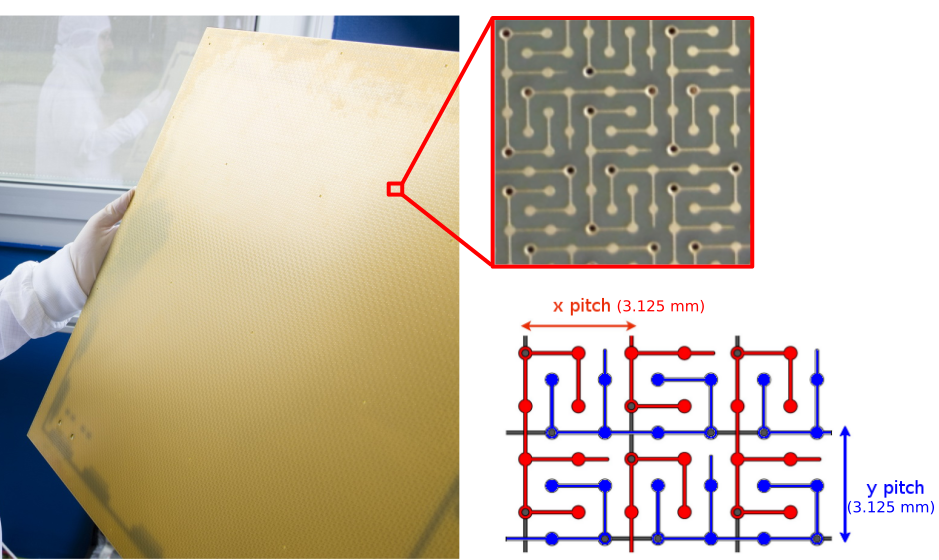
\includegraphics[width=0.7\textwidth]{anode.png} 
%          \column{.5\textwidth}
%          \textit{Text}
%        \end{columns}
%      \end{block}
%  \end{frame}


    \subsection[Tension et gain]{Tenue en tension et gain des LEMs}

    \begin{frame}{Tenue en tension des LEMs}
    	\begin{scriptsize}
    		\begin{center}
    			\textbf{Test des LEMs à la densité d'une DLArTPC dans une enceinte haute pression : stabilité en tension}\\
    			$G _{eff}= \mathcal{T}e^{A\textcolor{red}{\rho} d e^{-B\textcolor{red}{\rho}d/\textcolor{red}{V}}}$
    		\end{center} 
    		\begin{columns}
		    	\begin{column}{0.5\textwidth}
		    		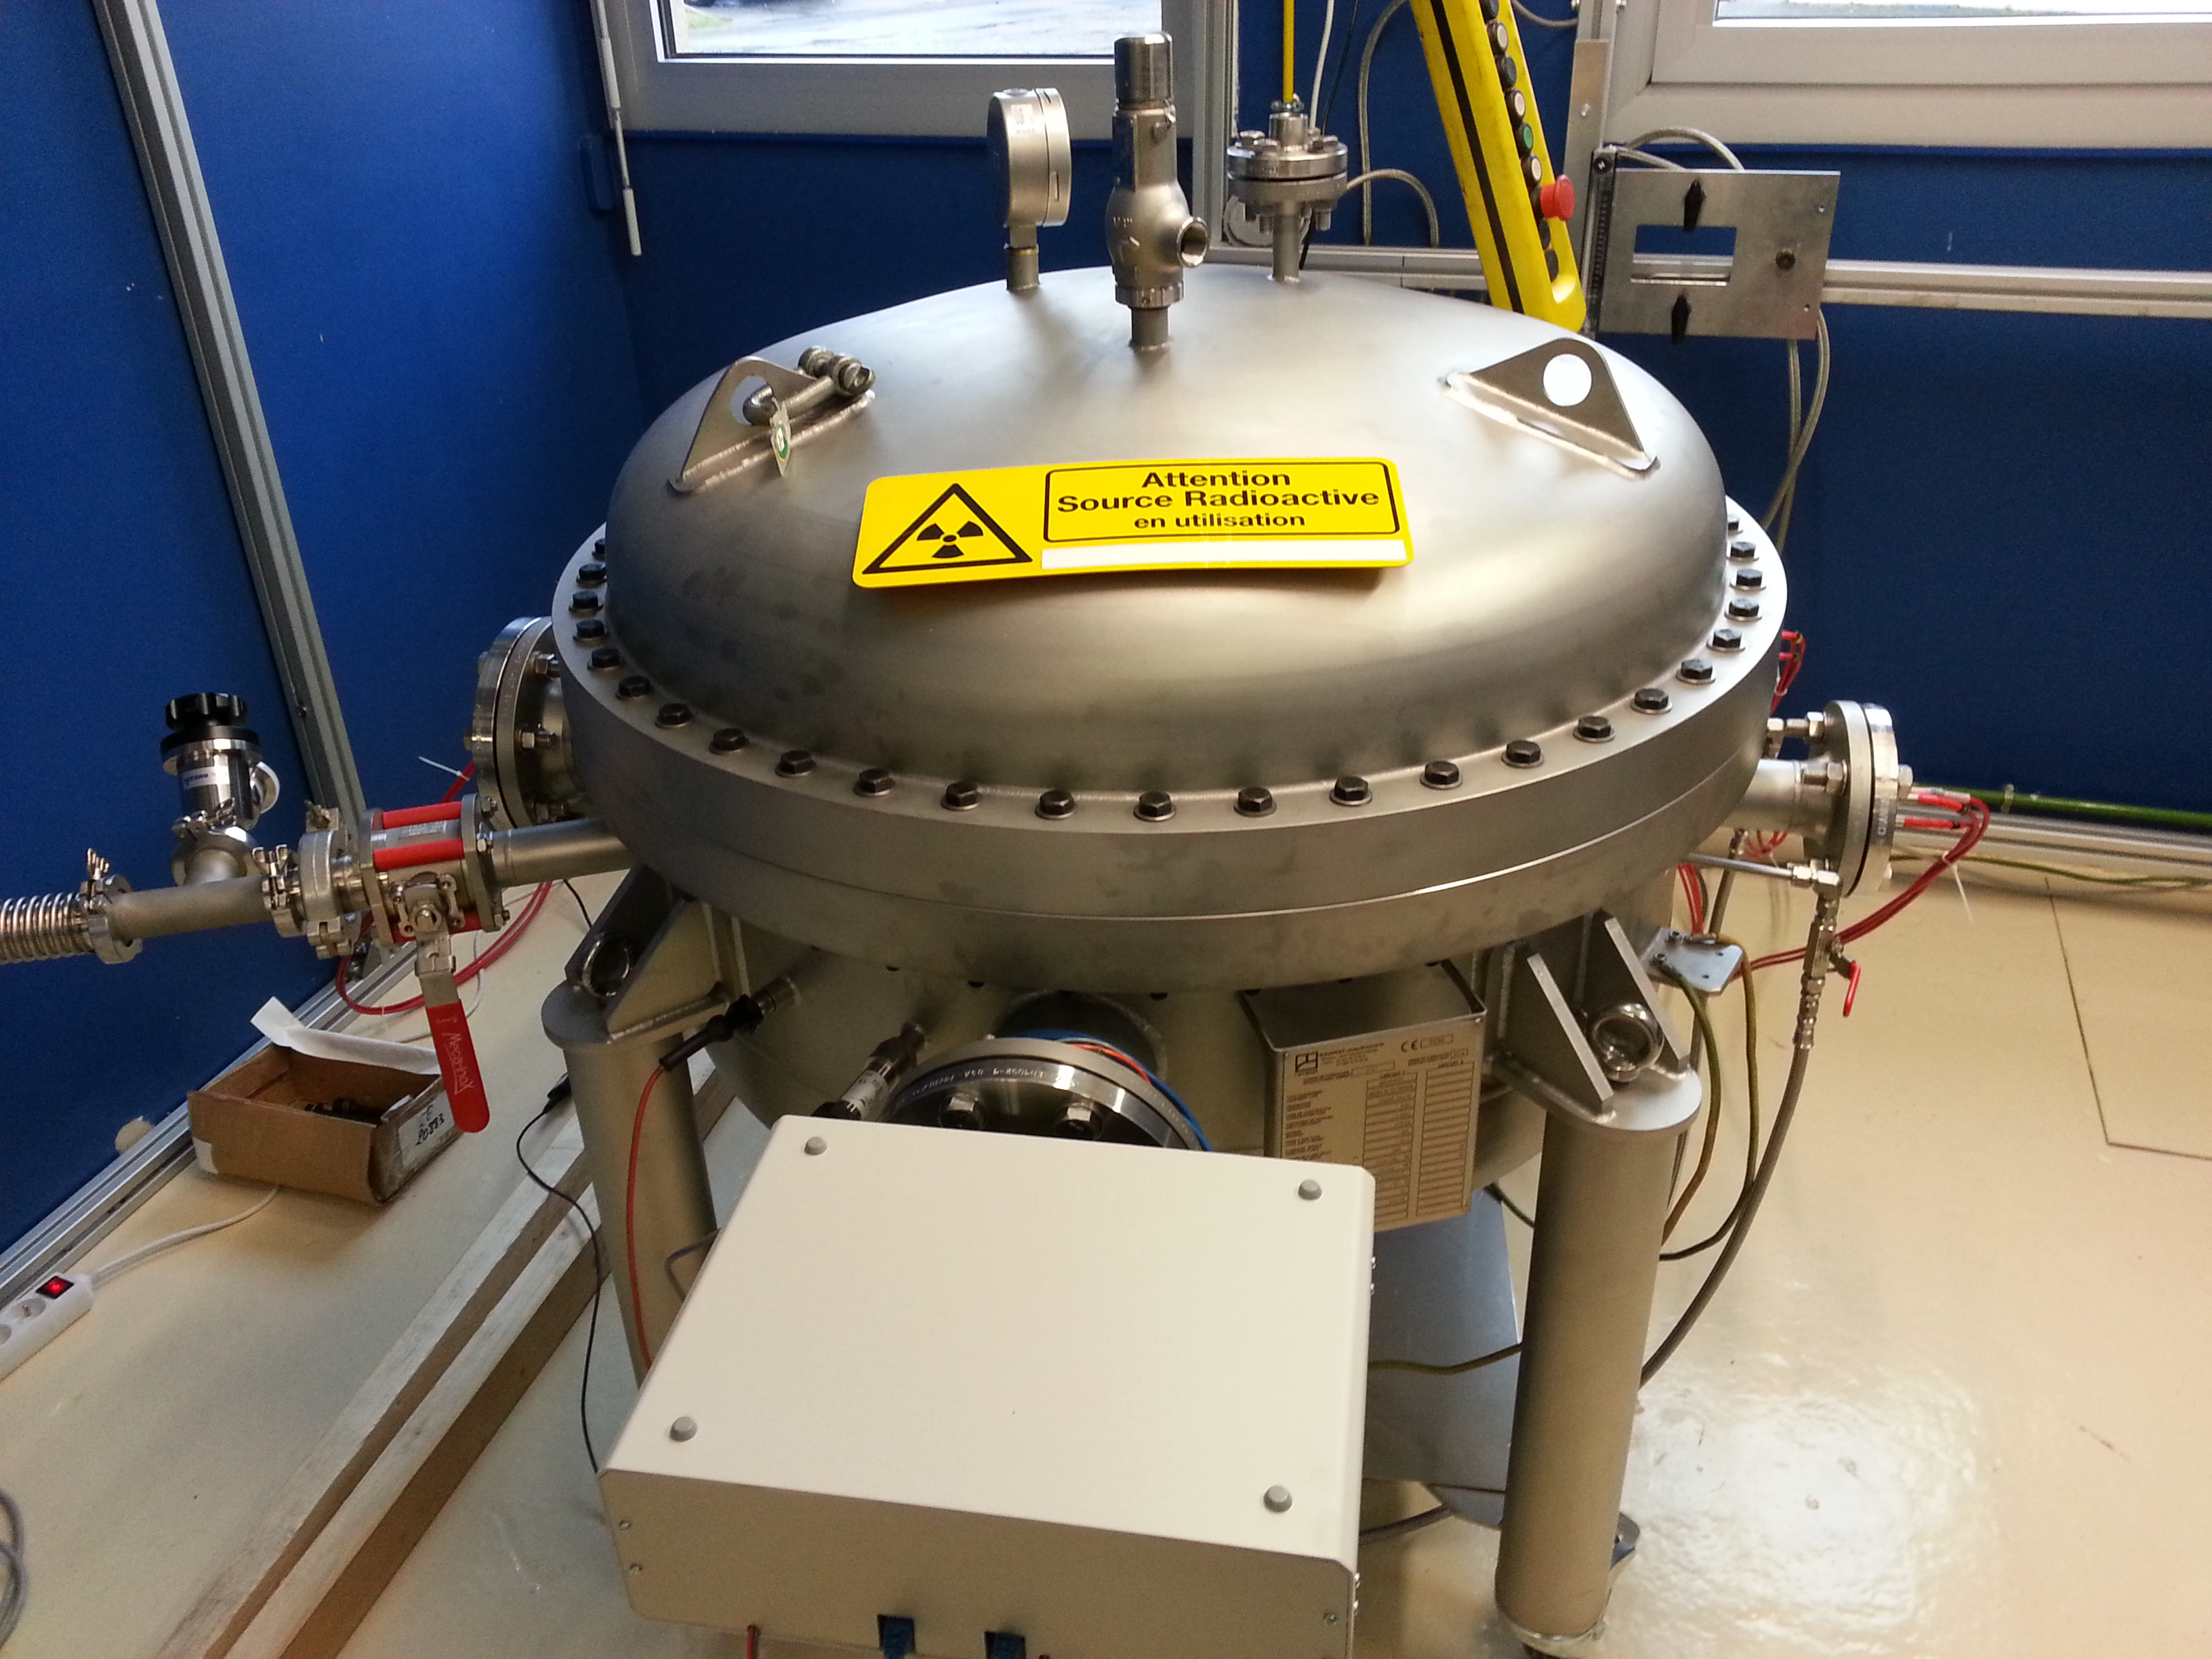
\includegraphics[height=3.7cm]{gamelle.jpg}\\
		    		\begin{itemize}
		    			\item $\rho \propto P/T$
		    			\item Pas de système cryo : \textcolor{red}{température ambiante}.
		    			\item Densité d'une DLArTPC à \textcolor{red}{\SI{3.3}{\bar}}.
		    		\end{itemize}
		    	\end{column}\hfill
		    	\begin{column}{0.5\textwidth}
		    		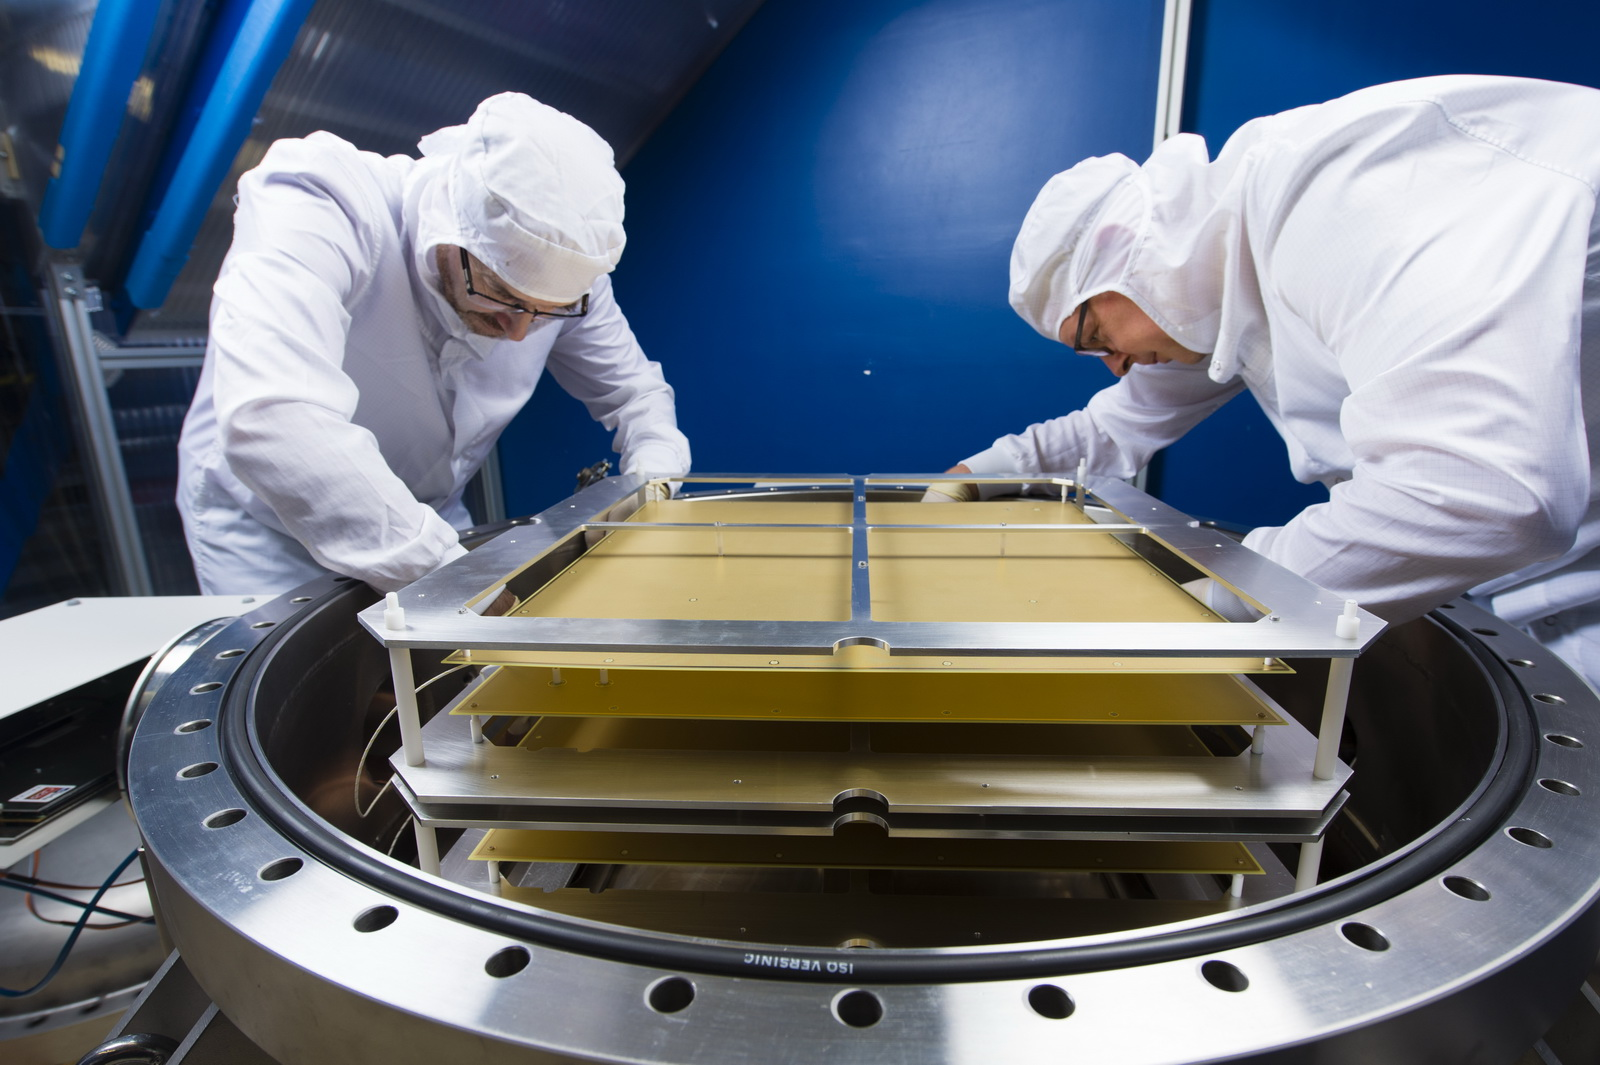
\includegraphics[height=3.7cm]{6lems_gamelle.jpg}\\
		    		\begin{itemize}
		    			\item Enceinte haute pressions: remplie d'argon gazeux.
		    			\item Empilement de 6-9 LEMs.
		    			\item A testé plus de 100 LEMs.
		    		\end{itemize}
		    	\end{column}
		    \end{columns}
	    \end{scriptsize} 
    \end{frame}

    \begin{frame}{Tenue en tension des LEMs}
   		\begin{columns}
    		\begin{column}{0.5\textwidth}
    			\begin{center}
	    			\begin{scriptsize}
		    			CFR-34 à 33--\SI{35}{\kilo\volt\per\centi\meter}\\
		    			\textcolor{red}{$\sim$ 20 décharges par heure}\\
		    		\end{scriptsize}
	    			\begin{tiny}
		    			(Design fait par \textbf{ETHZ}, utilisé dans le \TOO{})
		    		\end{tiny}\\
	    			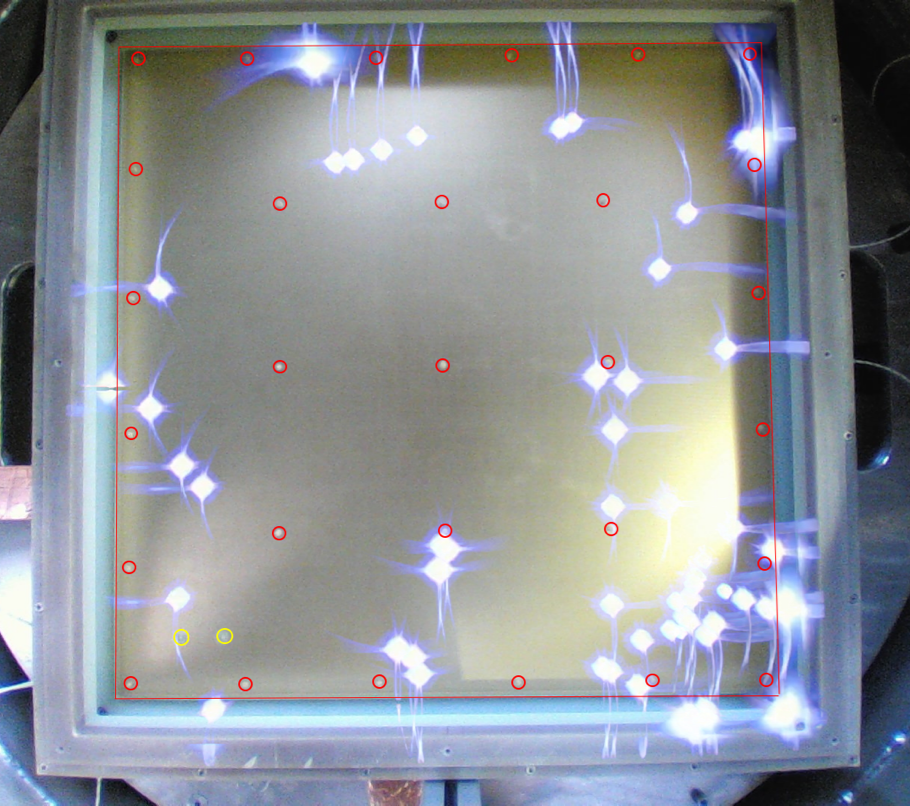
\includegraphics[height=3.1cm]{sparks_34.png}
    			\end{center}
    		\end{column}\hfill
    		\begin{column}{0.5\textwidth}
    			\begin{center}
	    			\begin{scriptsize}
		    			CFR-35 à \SI{35}{\kilo\volt\per\centi\meter} \\
		    			\textcolor{red}{$\sim$ 3 décharges par heure}\\
		    		\end{scriptsize}
	    			\begin{tiny}
	    				(Design fait par le \textbf{CEA}, utilisé dans le \SSS{})
	   				\end{tiny}\\
	    			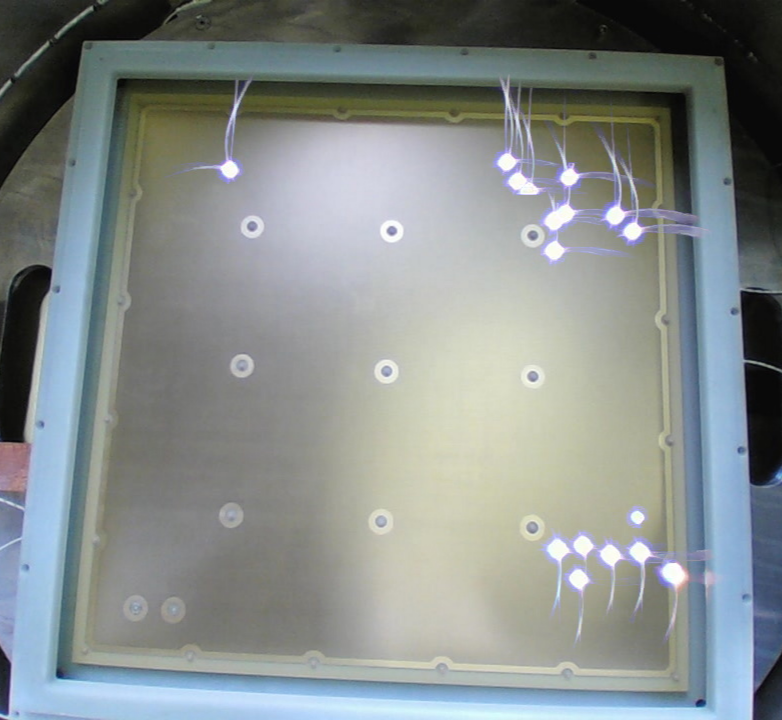
\includegraphics[height=3.1cm]{sparks_35.png}
	    		\end{center}
    		\end{column}
    	\end{columns}\vspace{0.1cm}
    	\begin{columns}
    		\begin{column}{0.5\textwidth}
    			\begin{scriptsize}
	    			\begin{itemize}
	    				\item CFR-34 instable au delà de \SI{32}{\kilo\volt\per\centi\meter}.
	    				\item Décharges surtout sur les bords et les coins.
	    			\end{itemize}
	    			\begin{itemize}
	    				\item[$\Rightarrow$] Nouveau design (CFR-35) avec bords plus grands. \textcolor{red}{(Solution temporaire)}
	    				\item[$\Rightarrow$] Nombre de décharges plus faible d'un ordre de grandeur.
	    			\end{itemize}
	    		\end{scriptsize}
    		\end{column}\hfill
    		\begin{column}{0.5\textwidth}
    			\begin{minipage}{0.48\textwidth}
    				\centering
    				\begin{scriptsize}
	    				CFR-34
	    			\end{scriptsize}
    				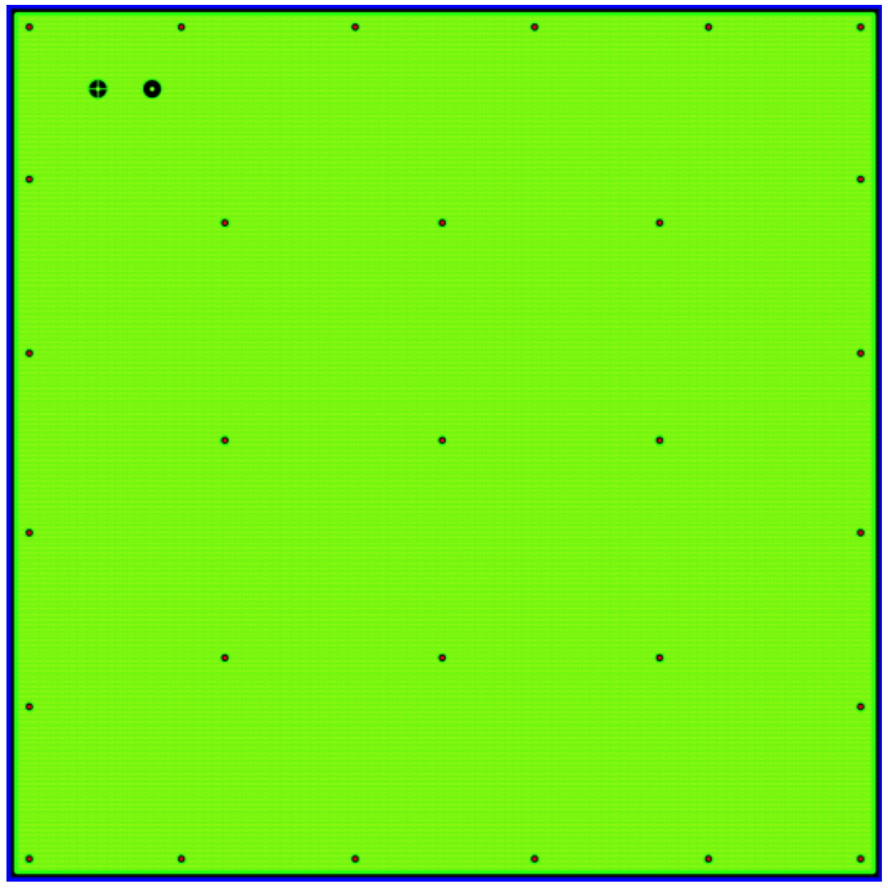
\includegraphics[width=.9\textwidth]{CFR-34.png}
    			\end{minipage}\hfill
    			\begin{minipage}{0.48\textwidth}
    				\centering
    				\begin{scriptsize}
	    				CFR-35
    				\end{scriptsize}
    				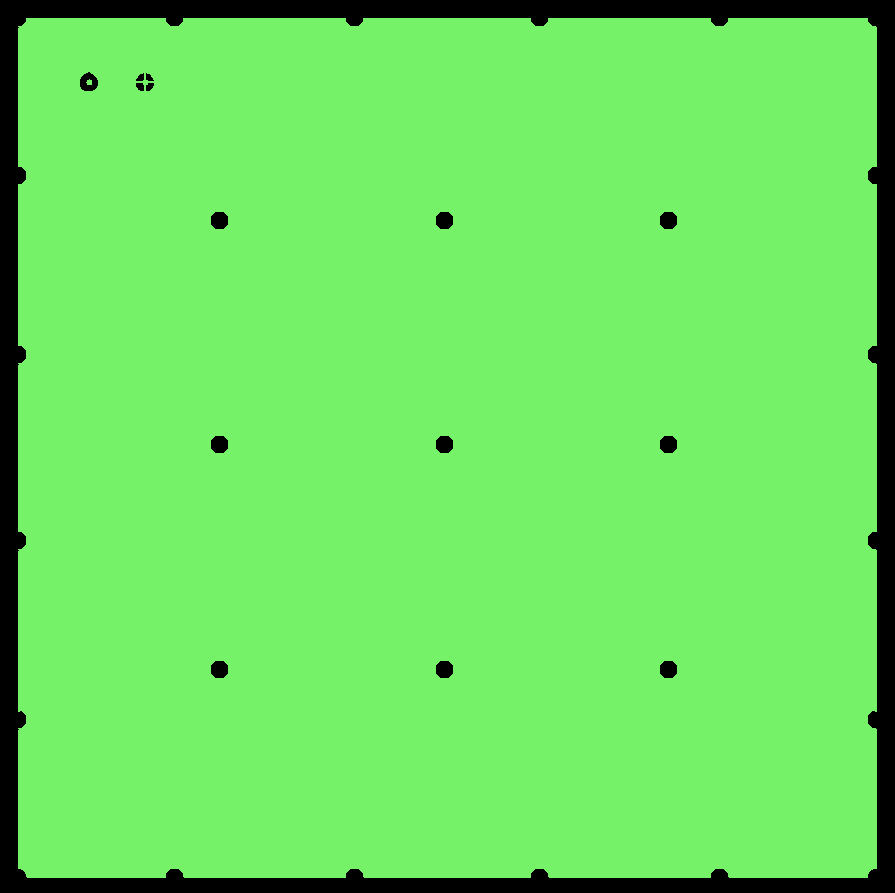
\includegraphics[width=.9\textwidth]{CFR-35.png}
    			\end{minipage}
    		\end{column}
    	\end{columns}
    \end{frame}

    \begin{frame}{Mesures de gain}
        %TODO mettre à jour
    	\begin{scriptsize}
%    		\begin{center}\textbf{Teste des LEMs à la densité d'une DLArTPC dans une enceinte haute pression : gain}\\\end{center}
    		\begin{columns}
    			\begin{column}{0.46\textwidth}
    				\centering 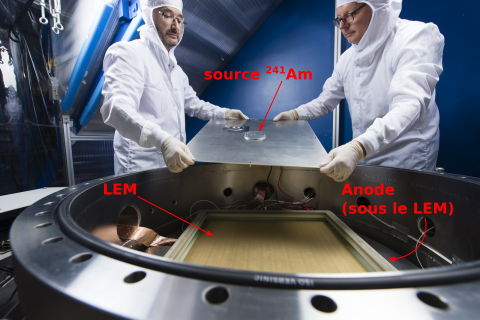
\includegraphics[width=\textwidth]{gamelle_source.png}
    			\end{column}\hfill
    			\begin{column}{0.58\textwidth}
    				\centering 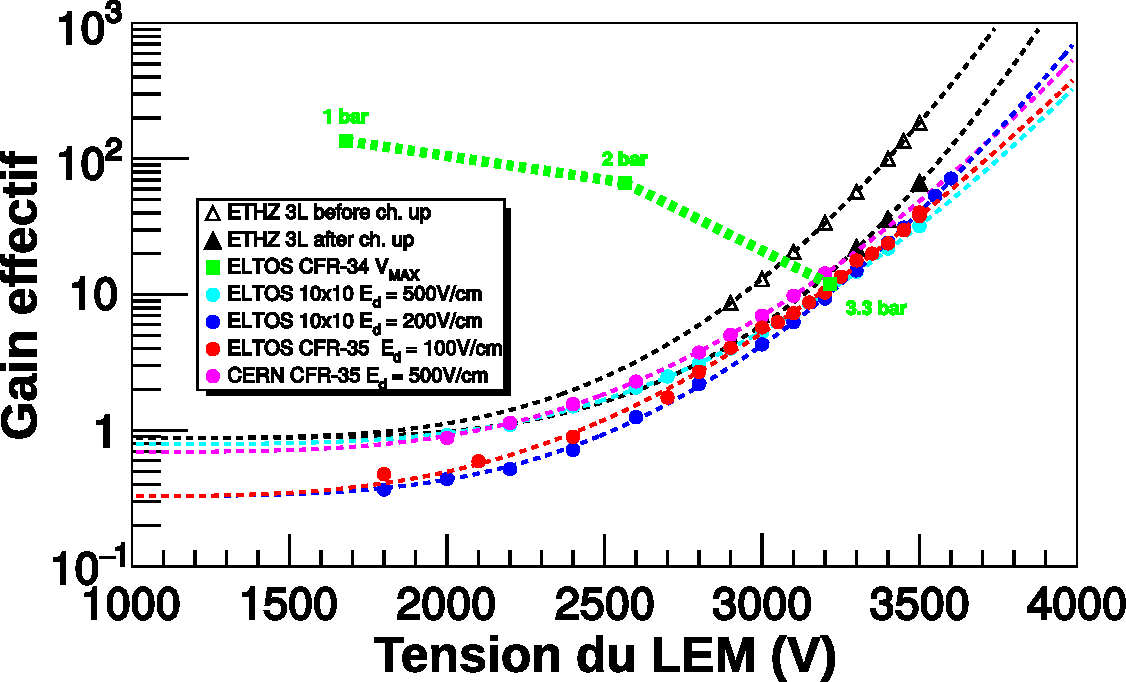
\includegraphics[width=\textwidth]{./pictures/New_LEM_Gain.pdf}
    			\end{column}
    		\end{columns}\vfill
    		\begin{columns}
    			\begin{column}{0.38\textwidth}
    				\begin{itemize}
    					\item 1 sandwich LEM-anode.
    					\item Source $^{241}$Am.
    					\item Peut mesurer le gain.
    				\end{itemize}
    			\end{column}\hfill
    			\begin{column}{0.58\textwidth}
    				\begin{itemize}
        				\item Bon accord avec les mesures du \SI{3}{\liter} après charging up.
    					\item LEMs de $10\times$\SI{10}{\centi\meter\squared} et $50\times$\SI{50}{\centi\meter\squared} se comportent de la même manière à haut gain.
    					\item Petites différences à faible gain.
    					\item  Gain max CFR--35 $>$ Gain max CFR--34
    				\end{itemize}
    			\end{column}
    		\end{columns}
%    		\vfill
%    		\textbf{$\Rightarrow$ Use CFR-35 for $\mathbf{6 \boldsymbol{\times} 6 \boldsymbol{\times} \SI[detect-weight]{6}{\meter\cubed}}$}.\\
    		%\textbf{Note:} Not sure about absolute gain value. Based on 3L measurements, CFR-35 should reach gain of $\sim$200.
    	\end{scriptsize}
    \end{frame}
    
    \subsection{Au CERN}

    {
    	\setlength\pdfpagewidth{12.8cm}%
    	\setlength\pdfpageheight{9cm}%
    	\usebackgroundtemplate{\includegraphics[width=\paperwidth]{CRP_bottom.png}}
    	\begin{frame}[plain]
    	\end{frame}
    }

    \begin{frame}{Boîte cryogénique au CERN (Juil. -- Déc. 2018)}
    	%the planarity obtained is within 1.2 mm over the entire plane (mail Dominique 21/09/2018)
   		\begin{columns}
   			\begin{column}{0.4\textwidth}
   				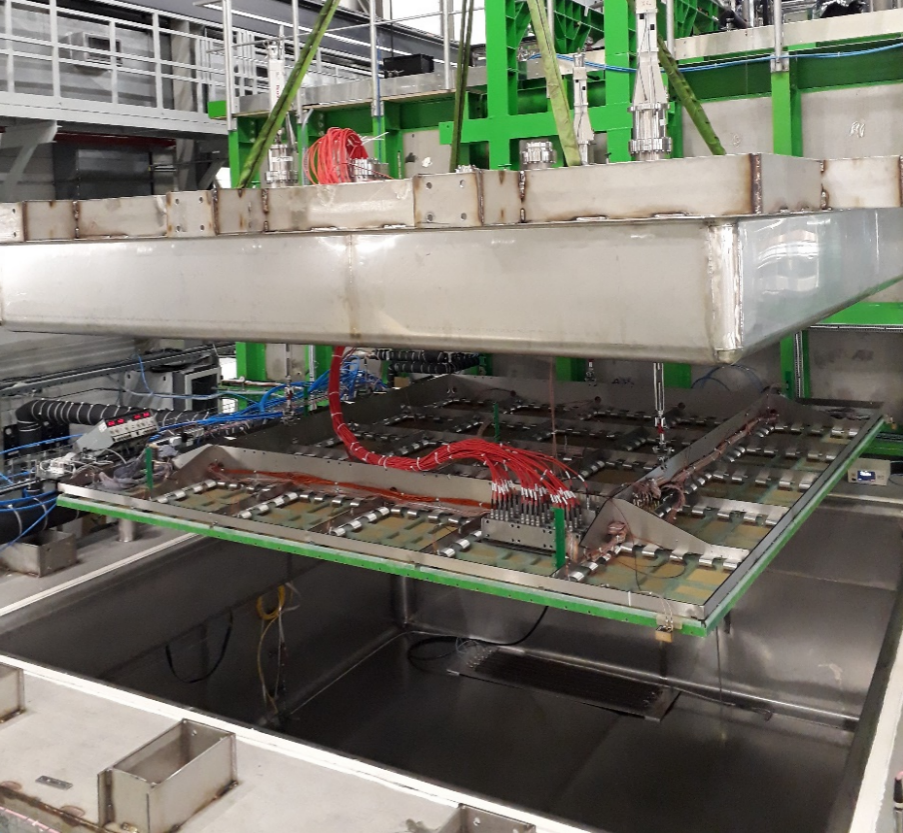
\includegraphics[width=\textwidth]{./pictures/crp_inserting_coldbox.png}\\
   				\includegraphics[width=\textwidth]{./pictures/in_coldbox.png}\\
   				CERN, bâtiment 182
    		\end{column}
    		\begin{column}{0.6\textwidth}
    			\begin{scriptsize}
	    			\textbf{Test des CRPs en condition double phase avant leur insertion dans le cryostat du \SSS{}.}\\
	    			
	    			\begin{itemize}
	    				\item \textbf{Tension maximum}
	    				\begin{itemize}
	    					\item Grille stable à la \textcolor{red}{valeur nominale de \SI{7.5}{\kilo\volt}}.
	    					\item LEMs stables à \textcolor{red}{3.0--\SI{3.1}{\kilo\volt}}\\
				    					$\Rightarrow$ Gain effectif estimé \textcolor{red}{$\geq 20$}.
	    				\end{itemize}
	    				\item \textbf{Stabilité (décharges par heure)}
	    				\begin{itemize}
	    					\item Stable sur plusieurs jours (semaines).
	    					\item \textcolor{red}{1 décharge par heure} par CRP (1 décharge en 36 heures par LEM): \textcolor{red}{ok pour DUN$\nu$E}.
	    					\item \textcolor{red}{1 décharge par heure} $\Rightarrow$ temps mort $\sim$0.3\%.
	    				\end{itemize}
	    				\item \textbf{Planéité}
	    				\begin{itemize}
	    					\item \textcolor{red}{$<$\SI{2}{\milli\meter}} à travers le CRP %: ok.
	    				\end{itemize}
	    			\end{itemize}
	    		\end{scriptsize}
    		\end{column}
    	\end{columns}
	    \end{frame}

%    \begin{frame}{Boîte cryogénique au CERN}
%        \includegraphics[width=\textwidth]{coldbox_current_voltage.pdf}
%        Rajouter une slide avec tension vs time, expliquer que les résultats sont bons
%    \end{frame}

       {
       	\setlength\pdfpagewidth{12.8cm}%
       	\setlength\pdfpageheight{11.5cm}%
       	\usebackgroundtemplate{\includegraphics[width=\paperwidth]{./pictures/fisheye.png}}
       \begin{frame}[plain]
       	
       \end{frame}
	    }

    \begin{frame}{Les grandes étapes}
        \begin{columns}
            \begin{column}{0.4\textwidth}
                \includegraphics[width=\textwidth]{./pictures/status_666.png}\\
                \includegraphics[width=\textwidth]{./pictures/crp_out_lar.png}\\
                \includegraphics[width=\textwidth]{./pictures/crp_in_lar.png}
            \end{column}\hfill
            \begin{column}{0.55\textwidth}
                \begin{itemize}
                    \item \textbf{Automne 2017 : Installation du cryostat à la plateforme neutrino}
                    \item\textbf{Printemps 2018} : Installation de la cage de dérive
                    \item \textbf{Hiver 2018 -- 2019} : Insertion des CRPs
                    \item \textbf{Mai 2019} : Fermeture
                    \item \textbf{Juin -- Juillet 2019} : Refroidissement et remplissage 
                    \item \textbf{Août 2019} : Mise en route
                    \item \textbf{Début septembre 2019} : 1ère traces
                \end{itemize}
            \end{column}
        \end{columns}
    \end{frame}
    
    {
       	\setlength\pdfpagewidth{12.8cm}%
       	\setlength\pdfpageheight{6.75cm}%
       	\usebackgroundtemplate{\includegraphics[width=\paperwidth]{./pictures/tracks_666.png}}
       \begin{frame}[plain]
             	
       \end{frame}
     }

    \section[Analyse du \SI{4}{\tonne}]{Simulations et analyses du prototype de \SI{4}{\tonne}}
    
    {
    	\usebackgroundtemplate{\includegraphics[width=\paperwidth]{./pictures/1.pdf}}
        \begin{specialframe}
            \vspace{2cm}\hspace*{-1.8cm}\parbox[t]{\textwidth}{
                \begin{center}
                    \begin{Huge}
                            \textcolor{pheniics_purple}{\textbf{\insertsection}}
                    \end{Huge}
                \end{center}
            }
        \end{specialframe}
    }

    \begin{frame}{Le prototype de \TOO{}}
		\begin{columns}
			\begin{column}{0.48\textwidth}
				\centering
				\includegraphics[width=0.8\textwidth]{311_2.png}
			\end{column}\hfill
			\begin{column}{0.48\textwidth}
				\begin{scriptsize}
					\textcolor{red}{A démontré le fonctionnement de DLArTPC à \SI{4}{\tonne}}
					Signal/Bruit $\sim$ 10 pour une MIP à une amplification de \SI{28}{\kilo\volt\per\centi\meter}.
				\end{scriptsize}
			\end{column}\hfill
		\end{columns}
		\centering
		\includegraphics[width=0.77\textwidth]{./pictures/events.png}\\
	\end{frame}
	    
    \begin{frame}{Le prototype de \TOO{}}
    	\begin{scriptsize}
    		\vfill
    		\begin{columns}
    			\begin{column}{0.35\textwidth}
    				Construit en 2016--2017, opéré entre Juin et Novembre 2017.\\
    				\vspace{0.3cm}
    				\textbf{But:} Tester les choix technologiques faits pour le \SSS{}.\\
    				\vspace{0.3cm}
    				\textbf{Difficultés rencontrées:} 
    				\begin{itemize}
    					\item Grille limitée à \SI{5}{\kilo\volt} (nominale : \SI{7}{\kilo\volt})
    					\item Haute tension à travers les LEMs instable
    					\item Déformation du CRP $\sim\SI{3}{\milli\meter}$
    				\end{itemize}
    				\textbf{$\Rightarrow$ Solutions apportées dans le \SSS{}} \\
    				\vspace{0.3cm}
    				\textbf{Analyse principale :} Gain (vs amplification, vs extraction, stabilité)\\
    				$\Rightarrow$ Utilise les muons cosmiques (MIP).
    			\end{column}\hfill
    			\begin{column}{0.65\textwidth}
    				\includegraphics[width=\textwidth]{./pictures/run840.png}\\
    			\end{column}
    		\end{columns}
	    \end{scriptsize}
    \end{frame}
    
    \begin{frame}{Lumière}
        \begin{scriptsize}
            \centering \includegraphics[width=0.7\textwidth]{./pictures/scintillation.pdf}\\\vfill
            \centering Deux sources de lumières dans une DLArTPC:
            \begin{columns}
                \begin{column}{0.5\textwidth}
                    Ionisation primaire :
                    \begin{itemize}
                        \item L'ionisation de l'argon produit une scintillation (\SI{128}{\nano\meter})
                        \item L'argon est transparent à cette lumière
                        \item Utilisée comme $t_0$
                    \end{itemize}
                \end{column}
                \begin{column}{0.5\textwidth}
                    Électroluminescence dans le gaz :
                    \begin{itemize}
                        \item Le passage d'électrons dans le gaz avec un champ de plus de \SI{2}{\kilo\volt\per\centi\meter} produit de l'électroluminescence
                        \item Informe sur le gain et la pureté (N$_2$)
                    \end{itemize}
                \end{column}
            \end{columns}
        \end{scriptsize}
    \end{frame}

    \subsection{Méthode d'analyse}

    \begin{frame}{Mesure du gain avec des muons cosmiques}
    	\begin{scriptsize}
            \begin{columns}
                \begin{column}{0.6\textwidth}
                    \centering \includegraphics[width=\textwidth]{langau.pdf}
                \end{column}\hfill
                \begin{column}{0.4\textwidth}
                    \begin{itemize}
       					\item Muon cosmique : MIP \\ $\Rightarrow$ dépôt d'énergie attendu connu
       					\item Valeur la plus probable (MPV) = \SI{1.7}{\mega\electronvolt\per\centi\meter}
       					\item Après recombinaison avec les ions (loi de Birks) : \SI{8.26}{\femto\coulomb\per\centi\meter}
       					\item $G_{eff}=\frac{MPV_0 + MPV_1}{MPV_{attendue}}$
       				\end{itemize}
                \end{column}
            \end{columns}
            \vspace{0.2cm}
            Calibration de l'électronique du \TOO{} $\Rightarrow$ conversion ADC$\times$temps$\to$\si{\femto\coulomb}
            \begin{center} \includegraphics[width=0.8\textwidth]{calibration.pdf} \end{center}
	    \end{scriptsize}
    \end{frame}

    \begin{frame}{Sélection des muons}
        \begin{scriptsize}
        \includegraphics[width=\textwidth]{highway.png}
        \begin{columns}
            \begin{column}{0.5\textwidth}
                \begin{itemize}
                    \item Muon : trace longue, droite et nette \\ $\Rightarrow$ Coupure sur $\frac{Q_A-Q_B}{Q_A} < 0.1$
                    \item Coupures supplémentaires : \begin{itemize}\begin{scriptsize}\item longueur $>\SI{50}{\centi\meter}$. \item \SI{2}{\degree} autour de la verticale, de l'horizontale, et des directions parallèle aux canaux des anodes.\end{scriptsize}\end{itemize}
                \end{itemize}
            \end{column}
            \begin{column}{0.5\textwidth}
                \hspace{0.3cm} Simulation Monte Carlo :
                \begin{itemize}
                    \item Efficacité de sélection des muons : 68\,\%
                    \item Échantillon final : 92\,\% de muons
                \end{itemize}
            \end{column}
        \end{columns}
        \end{scriptsize}
    \end{frame}
    
    \begin{frame}{Avec un champ d'amplification de \SI{28}{\kilo\volt\per\centi\meter}}
        \begin{scriptsize}
            \includegraphics[width=\textwidth]{./pictures/dQds_840.png}\\
            \begin{columns}[t]
                \begin{column}{0.5\textwidth}
                    \begin{itemize}
                        \item \textcolor{red}{$G_{eff}=1.8$}
                        \item Dans le \threeL{} après charging up : $G_{eff}=3.2$
                    \end{itemize}
                \end{column}
                \begin{column}{0.5\textwidth}
                    \begin{itemize}
                        \item Dans le \TOO{}, Extraction : \SI{1.8}{\kilo\volt\per\centi\meter}, Induction : \SI{1.5}{\kilo\volt\per\centi\meter}
                        \item Dans le \threeL{}, Extraction : \SI{2.5}{\kilo\volt\per\centi\meter}, Induction : \SI{5}{\kilo\volt\per\centi\meter}
                    \end{itemize}
                \end{column}
            \end{columns}
            \vfill
            \TOO{} et \threeL{} : différents champs d'extraction et d'induction\\
        \end{scriptsize}
    \end{frame}

    \subsection[Efficacités de collection]{Efficacités de collection}

    \begin{frame}{Simulation : efficacités de collection}
    	\begin{scriptsize}
    		\begin{columns}
    			\hspace{-1.5cm}
	    		\begin{column}{0.3\textwidth}
	    			$G_{eff} = \mathcal{T}e^{A\rho d e^{-B\rho d/V}}$\\
	    			$\mathbf{\mathcal{T}=G_{LEM}\boldsymbol{\times}\boldsymbol{\epsilon}_{ext} \boldsymbol{\times}\textcolor{red}{\epsilon_{LEM}}\boldsymbol{\times} \textcolor{blue}{\epsilon_{anode}}}$\\
	    			\vspace{0.6cm}
	    			\textbf{Difficulté rencontrée dans le $\mathbf{3 \times 1 \times \SI[detect-weight]{1}{\meter\cubed}}$:} Tension de la grille d'extraction limitée à \SI{5}{\kilo\volt}\\
	    			\vspace{0.3cm}
	    			$\Rightarrow$ N'a pas pu opérer à champ d'extraction et d'induction fixés.\\
	    			$\Rightarrow$ Besoin de connaître l'\textcolor{red}{impact} de ces champs \textcolor{red}{sur la collection de charge : }\\
	    			\begin{itemize}
                        \item Pour comparer \TOO{} et \threeL{}
                        \item Pour étudier gain vs amplification
                    \end{itemize}
%	    			\vspace{0.3cm}	    			
%		    		$\mathbf{G_{eff} = G_{LEM}} $ \\\hspace{0.7cm} $\boldsymbol{\times \epsilon}_{\mathbf{extraction}}$ \\\hspace{0.7cm} \textcolor{red}{$\boldsymbol{\times} \mathbf{P_{LEM}}$}\\\hspace{0.7cm} \textcolor{blue}{$\boldsymbol{\times} \mathbf{P_{Anode}}$}
	    		\end{column}\hfill\hspace{-3.2cm}
	    		\begin{column}{0.65\textwidth}
%	    			\flushright
	    			\includegraphics[width=1.18\textwidth]{./pictures/coll_proba_2.png}\\
	    		\end{column}
	    	\end{columns}
    	\end{scriptsize} 
    \end{frame}
    
    \begin{frame}{Outils de simulation}
        \begin{scriptsize}
            \begin{columns}
                \begin{column}{0.5\textwidth}
                    \includegraphics[width=\textwidth]{ansys_geom.png}
                \end{column}\hfill
                \begin{column}{0.5\textwidth}
                    \includegraphics[width=\textwidth]{./pictures/losses_with_lem.png}
                \end{column}
            \end{columns}
            \begin{columns}
                \begin{column}{0.5\textwidth}
                    \begin{itemize}
                        \item Champ à travers le CRP simulé avec ANSYS (éléments finis)
                        \item Défini un élément de base de la géométrie en nid d'abeille, conditions de symétrie pour générer toute la géométrie
                    \end{itemize}
                \end{column}
                \begin{column}{0.5\textwidth}
                    \begin{itemize}
                        \item Cartes de champs intégrées dans GarField : simulation de dérive des électrons à travers le CRP
                        \item Capable de retracer le parcours microscopique des électrons dans l'argon gazeux
                    \end{itemize}
                \end{column}
            \end{columns}
        \end{scriptsize}
    \end{frame}
    

    \begin{frame}{Simulation : efficacités de collection}
        \hbox{
     		$\mathbf{G_{eff}=G_{LEM}\boldsymbol{\times}\boldsymbol{\epsilon}_{extr} \boldsymbol{\times}\textcolor{red}{\epsilon_{LEM}}\boldsymbol{\times} \textcolor{blue}{\epsilon_{anode}}}$
     	}\vspace{0.2cm}
   		\begin{columns}
            \begin{column}{0.5\textwidth}
                \centering $\textcolor{red}{\epsilon_{LEM}}$
                \includegraphics[width=\textwidth]{./pictures/eff_lem_alone.pdf}
            \end{column}\hfill
            \begin{column}{0.5\textwidth}
                \centering $\textcolor{blue}{\epsilon_{Anode}}$
                \includegraphics[width=\textwidth]{eff_anode.pdf}
            \end{column}
        \end{columns}
   		\begin{columns}
            \begin{column}{0.5\textwidth}
                \begin{scriptsize}
                    \begin{itemize}
                        \item Dépend du champ dans le gaz entre l'interface et le LEM
                        \item Champ calculable à partir de la tension grille--LEM et de la position de l'interface
                    \end{itemize}
                \end{scriptsize}
            \end{column}\hfill
            \begin{column}{0.5\textwidth}
              \begin{scriptsize}
                \begin{itemize}
                    \item Dépend du charging up du LEM
                    \item Simulée ici avant charging up.
                \end{itemize}
              \end{scriptsize}
            \end{column}
        \end{columns}
    \end{frame}
    
    \begin{frame}{Efficacités de collection : mesures dans l'enceinte haute pression}
        \begin{scriptsize}
            $\mathbf{ \textcolor{red}{\epsilon_{LEM}}}$ et $\mathbf{ \textcolor{blue}{\epsilon_{anode}}}$ sont corrélées : valeurs individuelles pas mesurables. Mais \textbf{effets} individuels mesurables.\\
            $\Rightarrow$ Mesure de $G$ vs $E_{extr}$ et $E_{ind}$, puis normalisation aux efficacités simulées.
        \begin{columns}
            \begin{column}{0.5\textwidth}
                \centering $\textcolor{red}{\epsilon_{LEM}}$
                \includegraphics[width=\textwidth]{eff_lem_gamelle.pdf}
            \end{column}\hfill
            \begin{column}{0.5\textwidth}
                \centering $\textcolor{blue}{\epsilon_{Anode}}$
                \includegraphics[width=\textwidth]{eff_anode_gamelle.pdf}
            \end{column}
        \end{columns}
   		\begin{columns}
            \begin{column}{0.5\textwidth}
                \begin{itemize}
%                    \item Pas d'efficacité d'extraction (pas de liquide)
%                    \item Champ maximum limité par la distance Cathode-LEM et l'alimentation HT
                    \item Comportement similaire entre \SI{1}{\kilo\volt\per\centi\meter} et \SI{1.5}{\kilo\volt\per\centi\meter}
                \end{itemize}
            \end{column}\hfill
            \begin{column}{0.5\textwidth}
                \begin{itemize}
                    \item Comportement similaire, mais différences allant jusqu'à 15\,\%
                    \item[\danger] Mesures faites après charging up, simulations faites avant charging up!
                \end{itemize}
            \end{column}
        \end{columns}
        \end{scriptsize}
    \end{frame}

    \begin{frame}{Efficacités de collection : mesures dans le \TOO{}}
        \begin{scriptsize}
            \centering
            \includegraphics[width=0.75\textwidth]{./pictures/comp_311_eff.pdf}
            \vspace{0.2cm}
            \begin{columns}
                \begin{column}{0.5\textwidth}
                    \begin{itemize}
                        \item Champs d'amplification (\SI{28}{\kilo\volt\per\centi\meter}) et d'induction (\SI{1}{\kilo\volt\per\centi\meter}) constants
                        \item Grandes barres d'erreur à faibles champs dues aux imperfections de la planéité
                    \end{itemize}
                \end{column}
                \begin{column}{0.5\textwidth}
                    \begin{itemize}
                        \item MPV Normalisée à $\epsilon_{extr}$ à \SI{2}{\kilo\volt\per\centi\meter} pour comparer le comportement
                        \item La MPV divisée par  $\epsilon_{LEM}$ est meilleure que la MPV seule.
                    \end{itemize}
                \end{column}
            \end{columns}
        \end{scriptsize}
    \end{frame}

    \begin{frame}{Efficacités de collection : impact sur la précision du gain}
        \begin{center} \vspace{-0.5cm}\includegraphics[width=\textwidth]{CRP-metrologie.png} \end{center}
        \begin{scriptsize}
            \begin{columns}
                \begin{column}{0.6\textwidth}
                    \centering \includegraphics[width=\textwidth]{./pictures/extr_eff.pdf}
                \end{column}\hfill
                \begin{column}{0.4\textwidth}
                    \begin{itemize}
       					\item Déformation du CRP : $\pm\SI{1.8}{\milli\meter}$
       					\item[$\Rightarrow$]  25\,\% variation des champs entre la grille et l'interface et entre l'interface et les LEMs
       					\item Variation de $\epsilon_{extr}\times\epsilon_{LEM}$ à basse tension d'extraction
       				\end{itemize}
                     \textbf{Note : } dans le \SSS{},  $\Delta V$ Grille-LEM $\sim\SI{2.5}{\kilo\volt}\Rightarrow$ efficacité $\sim$ constantes.
                \end{column}
            \end{columns}
        \end{scriptsize}
    \end{frame}

    \begin{frame}{Stabilité du gain à travers le CRP dans le \TOO{}}
        \begin{scriptsize}
            \centering Deux runs à 12 heures d'intervalle. Extraction \SI{1.9}{\kilo\volt\per\centi\meter}, Amplification \SI{28}{\kilo\volt\per\centi\meter}, Induction \SI{1.5}{\kilo\volt\per\centi\meter}\\\vspace{0.2cm}
            \begin{center} \vspace{-0.5cm}\includegraphics[width=0.9\textwidth]{dQds_2D_840.pdf} \end{center}
            \begin{center} \vspace{-0.5cm}\includegraphics[width=0.9\textwidth]{dQds_2D_842.pdf} \end{center}
            \vspace{-0.5cm}
            \begin{itemize}
    			\item Variations attendues dues aux variations d'épaisseur et à la planéité du CRP : $\pm 12 \,\%$
    			\item Variations observées jusqu'à $\sim \pm15\,\%$ : compatibles
			\end{itemize}
        \end{scriptsize}
    \end{frame}

  \subsection{Charging up}

%    \begin{frame}{Charging up}
%    	\begin{scriptsize}
%    		\begin{columns}
%    			\begin{column}{0.5\textwidth}
%    				\includegraphics[width=0.85\textwidth]{CU.png}\\
%                    \vspace{0.1cm}
%    				\includegraphics[width=\textwidth]{3L_charging_up.png}\\
%    				\includegraphics[width=0.7\textwidth]{gain_3L.pdf}
%    			\end{column}\hfill
%    			\begin{column}{0.5\textwidth}
%    				\begin{itemize}
%    					\item Lignes de champ traversent le FR4\\
%    					$\Rightarrow$ L'accumulation d'électron \textcolor{blue}{déforme et atténue} le champ
%    					\item Charging up: \textcolor{red}{$G_{eff}(t)$ décroît} jusqu'à un plateau.
%%    					\item Le temps de charging up time dépend de la tension dans le LEM et du taux de dépôt de charge.
%    				\end{itemize}
%    				\vspace{0.3cm}
%    				\begin{itemize}
%    					\item Simulation de $\textcolor{blue}{\epsilon_{Anode}}$ suppose un LEM \textcolor{red}{avant charging up}
%    					\item Mesures de gain dans l'enceinte faites \textcolor{red}{après charging up}
%    					\item Mesures de gain dans le \TOO{} faites \textcolor{red}{pendant le charging up}
%    					\item[$\Rightarrow$] $\textcolor{blue}{\epsilon_{Anode}}$ simulée sera plus faible que dans le \TOO{} (moins de pertes dues au charging up). Mais ce qui compte vraiment est le \textbf{comportement} de $\textcolor{blue}{\epsilon_{Anode}}$
%    				\end{itemize}
%    			\end{column}
%    		\end{columns}
%    	\end{scriptsize}
%    \end{frame}

   \begin{frame}{Charging up dans le \TOO{}}
        \begin{scriptsize}
            \includegraphics[width=\textwidth]{charging_up.png}
            \begin{itemize}
                \item Charging up $\sim$ linéaire sur les durées des runs du \TOO{}
                \item Persiste une fois la tension coupée
            \end{itemize}
        \end{scriptsize}
    \end{frame}

  \subsection{Zones mortes}
    
    \begin{frame}{Simulations : zones mortes}
    	\begin{scriptsize}
    		\begin{minipage}{0.38\textwidth}
    			\begin{center}
    				\includegraphics[width=0.8\textwidth]{corner_annotations.png}\\
    				design : CFR-34\\
    			\end{center} 
    			Zones mortes = zones sans trous d'amplification:
    			\begin{itemize}
    				\item Bords du LEM
    				\item Trous des vis.
    				\item Connecteurs haute tension.
    			\end{itemize}
    			$\Rightarrow$ Collection de charge?\\
    			$\Rightarrow$ Résolution en énergie?\\
    			
    			\textbf{ANSYS} simule la carte de champ à travers le CRP.\\
    			\textbf{GarField} simule la dérive des électrons dans cette carte.\\
    		\end{minipage}
    		\begin{minipage}{0.58\textwidth}
    			\centering
    			\includegraphics[width=0.8\textwidth]{drift_example.png}\\
    			\vspace{0.5cm} \hspace{0.1cm}
    			\begin{minipage}{0.48\textwidth}
    				\centering
    				\textbf{Carte d'efficacité du LEM CFR-34}\\
    				\includegraphics[width=\textwidth]{eff_map.png}
    			\end{minipage}\hfill
    			\begin{minipage}{0.48\textwidth}
    				\centering
    				\textbf{Impact sur la charge collectée d'un événement électron}\\
    				\includegraphics[width=1.2\textwidth]{electron.png}
    			\end{minipage}
    		\end{minipage}
    	\end{scriptsize} 
    \end{frame}

    \begin{frame}{Zones mortes dans le \TOO{}}{MPV mesurée sur les bords des LEMs dans le \TOO{}}
        \begin{scriptsize}
            \begin{columns}
                \begin{column}{0.5\textwidth}
                    \includegraphics[width=\textwidth]{dQds_840_0_border.pdf}
                \end{column}
                \begin{column}{0.5\textwidth}
                    \includegraphics[width=\textwidth]{dQds_840_1_border.pdf}
                \end{column}
            \end{columns}
            \begin{columns}
                \begin{column}{0.5\textwidth}
                    \begin{itemize}
                        \item MPV sur les seconds canaux au dessus des bords (pas de coups dans les premiers canaux)
                        \item 35\,\% inférieure à la MPV mesurée sur les autres canaux.
                        \item Prédiction des simulations : 60\,\% inférieure
                    \end{itemize}
                \end{column}
                \begin{column}{0.5\textwidth}
                    \begin{itemize}
                        \item Simulation faite aux champs nominaux
                        \item Mesures faites à plus bas champs
                        \item[$\Rightarrow$] Champs électriques différents, peut expliquer la différence 
                    \end{itemize}
                \end{column}
            \end{columns}
        \end{scriptsize}
    \end{frame}

  \subsection{Gain vs amplification}

    \begin{frame}{Gain vs amplification}
        \begin{scriptsize}
            \centering \includegraphics[width=0.75\textwidth]{./pictures/gain_vs_ampli.pdf} \\
            \vspace{0.2cm}
            \begin{columns}
                \begin{column}{0.5\textwidth} 
                    \begin{itemize}
                        \item  \textcolor{red}{Bon accord avec le \threeL{} après charging up}
                        \item[$\Rightarrow$] Charging up complet.
                    \end{itemize}
                \end{column}
                \begin{column}{0.5\textwidth}
                    Petite différence avec \SI{3}{\liter} :
                    \begin{itemize}
                        \item Différences d'épaisseur? 
                        \item $\textcolor{blue}{\epsilon_{Anode}}$?
                    \end{itemize}
                \end{column}
            \end{columns}
        \end{scriptsize}
    \end{frame}
    
    \begin{frame}{Gain vs amplification}
        \begin{scriptsize}
            \centering \includegraphics[width=0.75\textwidth]{./pictures/gain_vs_ampli_circle.pdf} \\ 
            \begin{columns}
                \begin{column}{0.5\textwidth}
                    \textcolor{red}{Run au delà de \SI{28}{\kilo\volt\per\centi\meter}} : très grandes barres  d'erreurs 
                    \begin{itemize}
                        \item  Plus grand champ d'ampli $\Rightarrow$ plus grand impact des variations d'épaisseurs des LEMs
                         \item Plus faible champ d'extraction ($\sim \SI{1}{\kilo\volt\per\centi\meter}$) $\Rightarrow$ plus grand impact des imperfections de planéité
                    \end{itemize}
                \end{column}
                \begin{column}{0.5\textwidth}
                    \begin{itemize}
                        \item Faible champ d'extraction $\Rightarrow$ étalement en temps du signal.
                        \item[$\Rightarrow$] Difficultés de reconstruction
                        \item Développement d'un algorithme de reconstruction dédié
                    \end{itemize}
                \end{column}
            \end{columns}
        \end{scriptsize}
    \end{frame}
    
    \subsection{Reconstruction des runs à haute amplification}
    
    \begin{frame}{Problème lors de la suppression du bruit cohérent}
        
        \begin{scriptsize}
            \begin{columns}
                \begin{column}{0.45\textwidth}
                    \centering \textbf{Signal trouvé:}\\
                    \centering \includegraphics[width=\textwidth]{./pictures/good_pedsub.png}\\
                    \centering \includegraphics[width=\textwidth]{./pictures/good_cnsub.png}\\
                    \centering \textbf{Signal non trouvé:}\\
                    \centering \includegraphics[width=\textwidth]{pedsub_adcs_high_threshold.pdf}\\
                    \centering \includegraphics[width=\textwidth]{cnsub_adcs_high_threshold.pdf}\\
                 \end{column}
                \begin{column}{0.55\textwidth}
                    \textbf{Bruit cohérent = bruit commun à tous les canaux d'une même carte d'électronique.} \\\vspace{0.3cm}
                    Suppression du bruit cohérent :
                    \begin{itemize}
                        \item regroupement des canaux par groupe de 32
                        \item Calcul de la moyenne d'ADC pour chaque bin de temps
                        \item Soustraction de cette moyenne par bin de temps dans chaque canal d'ADC
                    \end{itemize} 
                    \vspace{0.3cm}
                    \textbf{ Exemple d'un canal d'ADC avant et après suppression du bruit cohérent dans le run à \SI{30}{\kilo\volt\per\centi\meter} }: \\Le coup n'est pas vue et n'est pas ignoré pour le calcul du bruit cohérent. \\
                     Suppression trop forte $\Rightarrow$ coup supprimé \\
                    $\Rightarrow$ Trace segmentée \\
                    $\Rightarrow$ Mauvaise reconstruction avec LArSoft \\
                \end{column}
            \end{columns}
        \end{scriptsize}
    \end{frame}

    \begin{frame}{Reconstruction avec LArSoft}
        \begin{scriptsize}
            \begin{columns}
                \begin{column}{0.65\textwidth}
                    \centering \textbf{Exemple de reconstruction, haute extraction}\\
                    \centering \includegraphics[width=\textwidth]{event_larsoft.png}
                \end{column}
                \begin{column}{0.35\textwidth}
                    \centering \textbf{Exemple de distribution $dQ/ds$, basse extraction}\\
                    \centering \includegraphics[width=\textwidth]{dQds_1197_0.pdf}
                \end{column}
            \end{columns}\vfill
            \begin{columns}
                \begin{column}{0.5\textwidth}
                    \textbf{Reconstruction avec LArSoft :}
                    \begin{enumerate}
                        \item Identification des région d'intérêts (ROI, potentiels dépôts de charges)
                        \item Nombreux passages de suppression de bruit
                        \item Identifications des coups dans chaque vue séparément et regroupements en amas 2D
                        \item Identification des amas 3D et calcul de $dQ/ds$
                    \end{enumerate}
                \end{column}
                \begin{column}{0.5\textwidth}
                    $\Rightarrow$ Si trop de coups sont ignorés, la trace est segmentée et de nombreuses petites traces sont reconstruites\\
                    $\Rightarrow$ Mauvaise identifications des amas 3D et mauvais calcul de $ds$, et donc de $dQds$
                \end{column}
            \end{columns}
        \end{scriptsize}
    \end{frame}
    
    \begin{frame}{Solution : transformation de Hough}
        \textbf{Paramétrisation d'une droite }: $r=x\cos(\theta)+y\sin(\theta)$\\
        \textbf{Calcul de $\boldsymbol{r}$ pour $\boldsymbol{\theta\in[0,\pi]}$} : un point dans un repère cartésien correspond à une sinusoïdale dans l'espace de Hough.\\
        $\Rightarrow$ Un ensemble de points sur une même droite dans un repère cartésien correspond à un point dans l'espace de Hough.\\
        $\Rightarrow$ \textcolor{red}{Trouver une droite revient à trouver un maximum local}.\\\vfill
        \includegraphics[width=\textwidth]{./pictures/HT.pdf}
    \end{frame}

    \begin{frame}{Reconstruction avec la transformation de Hough}
        \begin{scriptsize}
            \begin{columns}
                \begin{column}{0.5\textwidth}
                    \textbf{Nouvelle méthode de reconstruction :}
                    \begin{enumerate}
                        \item Identification des ROI
                        \item Un passage de suppression de bruit cohérent
                        \item Identifications des coups
                        \item \textbf{Transformation de Hough} : \textcolor{red}{cherche des droites et non des segments}
                        \item \textbf{Seconde suppression du bruit sachant où sont les traces}, calcul de $dQ/ds$
                    \end{enumerate}
                    $\Rightarrow$ Une trace segmentée peut être reconstruite
                \end{column}
                \begin{column}{0.5\textwidth}
                    \centering \includegraphics[width=0.8\textwidth]{HT_real_data.pdf}
                \end{column}
            \end{columns}
            \begin{center} \includegraphics[width=0.8\textwidth]{HT_real_data_track.pdf} \end{center}
        \end{scriptsize}
    \end{frame}

    \begin{frame}{Reconstruction avec la transformation de Hough}
        \begin{scriptsize}
            \begin{center} \includegraphics[width=0.8\textwidth]{cnsub_fromtrack.pdf} \end{center}
            \begin{columns}
                \begin{column}{0.6\textwidth}
                    Transformation de Hough\\
                    \includegraphics[width=\textwidth]{1197_dQds_0.pdf}
                \end{column}
                \begin{column}{0.4\textwidth}
                    LArSoft\\
                    \includegraphics[width=\textwidth]{dQds_1197_0.pdf}
                \end{column}
            \end{columns}
        \end{scriptsize}
    \end{frame}

%    \begin{specialframe}
%        \hspace*{-1.8cm}\parbox[t]{\textwidth}{
%            \centering \begin{Huge}
%            \textbf{Conclusion}
%            \vspace{2cm}
%            \end{Huge}
%            \begin{itemize}
%                \item Principe de la DLArTPC \textcolor{green}{\checkmark} à \SI{4}{\tonne}
%                \item[$\Rightarrow$] Tenu en tension grille et LEMs : problèmes réglés dans le \SSS{}
%                \item \SSS{} : début d'opération prometteur
%            \end{itemize}
%            \vspace{0.3cm}
%            \textbf{À suivre :}
%            \begin{itemize}
%                \item Gain $> 20$?
%                \item Pureté?
%                \item Stabilité?
%            \end{itemize}
%        }
%    \end{specialframe}
    {
        \usebackgroundtemplate{\includegraphics[width=\paperwidth]{./pictures/1.pdf}}
        \begin{specialframe}
            \hspace*{-1.8cm}\parbox[t]{\textwidth}{
                        \centering \begin{Huge}
                        \vspace{2cm}
                        \textbf{Conclusion}
                        \vspace{1cm}
                        \end{Huge}
                        \begin{itemize}
                            \item Principe de la DLArTPC \textcolor{green}{\checkmark} à \SI{4}{\tonne}
                            \item[$\Rightarrow$] Tenu en tension grille et LEMs : solutions apportées dans le \SSS{}
                            \item \SSS{} : début d'opération prometteur, premières traces observées
                        \end{itemize}
                        \vspace{0.3cm}
                        \textbf{À suivre :}
                        \begin{itemize}
                            \item Gain $> 20$?
                            \item Pureté?
                            \item Stabilité?
                        \end{itemize}
                    }
        \end{specialframe}
    }
    
\end{document}
